\chapter{Muon System Timing \label{sec:timing}}

\section{Foreword}
This chapter details the measurement of the arrival time of particles in the muon system of CMS. A particular focus is put on the measurement in the CSC system
with a description of the measurements in the whole of the muon system given at the end. 

\section{Introduction}
Muons coming from collisions in the LHC take approxiamtely 25-40ns to travel from the interaction point to the muon system. As CMS was designed to collect data with protons
colliding every 25ns the time of flight (TOF) of muons is a significant time interval. The muon system must be able to associate tracks in the system to the
correct bunch crossing window for the L1 trigger.
This is required to trigger the readout of the data in the rest of the detector associated with the collsion that the track came from.
The method to determine timing synchronization of the CSC subsystem is described below.

Additionally, the timing in the muon system can be used to separate out different sources of tracks. These sources include collision muons from the
triggered bunch crossing wondow, muons from adjacent bunch crossing windows, muons from cosmic rays, and possibly 
HSCPs predicted in theories of new physics. To do this the time of hits in the muon system is measured and a combined time for each track is calculated.

\section{CSC Hit Timing}
Hits in the CSCs are found from a combination of signals from the anode wires and cathode strips. Both of the signals can be used to estimate the time of the hits.

Time is measured by the cathode strips in two ways, one for online use in the L1 trigger and one for offline measurement. The online measurement finds the peak of the
charge distribution and associates it with the particular bunch crossing window. For offline determination of the position and 
time of the hits, the charge on cathode strips is sampled every 50ns.
The time of the hits is estimated with a fit to the charge distribution. Calibration constants are subtracted from the times during reconstruction to center the times at zero.
The constants are found for each chamber and are derived from times associated with high quality, high momentum muons. Cathode times have a resolution of approxiamtely 7.0ns.

As stated in Section~\ref{sec:subsystems}, signals from the anode wires are passed to a constant fraction discriminator which outputs a 40ns pulse
that is then digitized every 25ns. Depending on when the pulse starts, the hit can have either one or two bits being high. Given the same
first high bit, it can be inferred that hits with the next bit low arrived earlier than hits with the next bit high.
Hits with only one high bit are estimated to have arrived at the time of that bit while those with two high are estiamted to be from the average of the two bits.
Thus, it is possible to estimate the time of anode hits with a 12.5 ns quantization. The anode times are calibrated to have a mean of zero in the same method as
per the cathode times. The resolution of the anode hit timing is approximately 8.6 ns 

The distribution of the time of anode and cathode hits associated with high quality, high momentum muons is shown in Fig~\ref{fig:hittime}.
As can be seen in the right plot the anode time has a large tail of positive times. This is dealt with by a cleaning procedure defined below.

\begin{figure}
  \begin{center}
      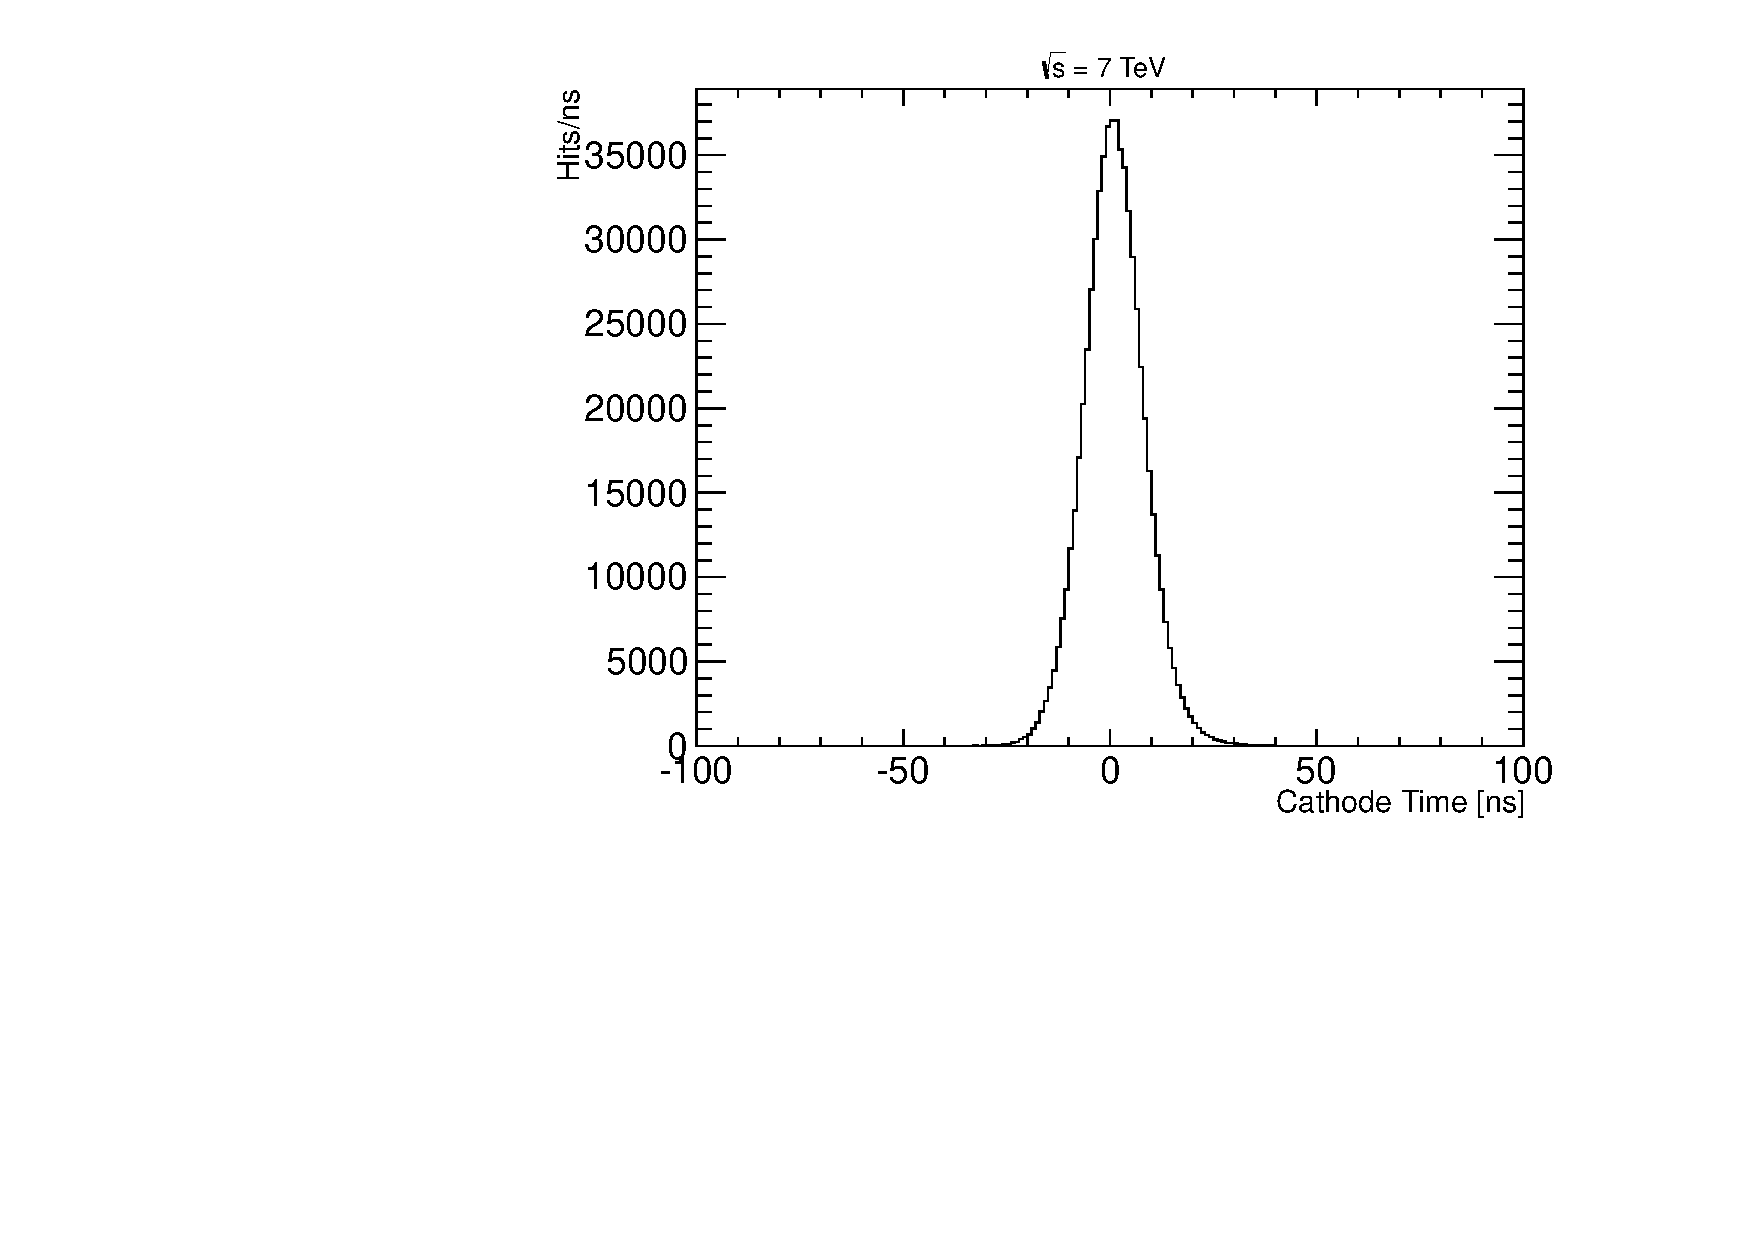
\includegraphics[clip=true, trim=0.0cm 0cm 2.0cm 0cm, width=0.44\textwidth]{figures/timing/CathodeTime}
      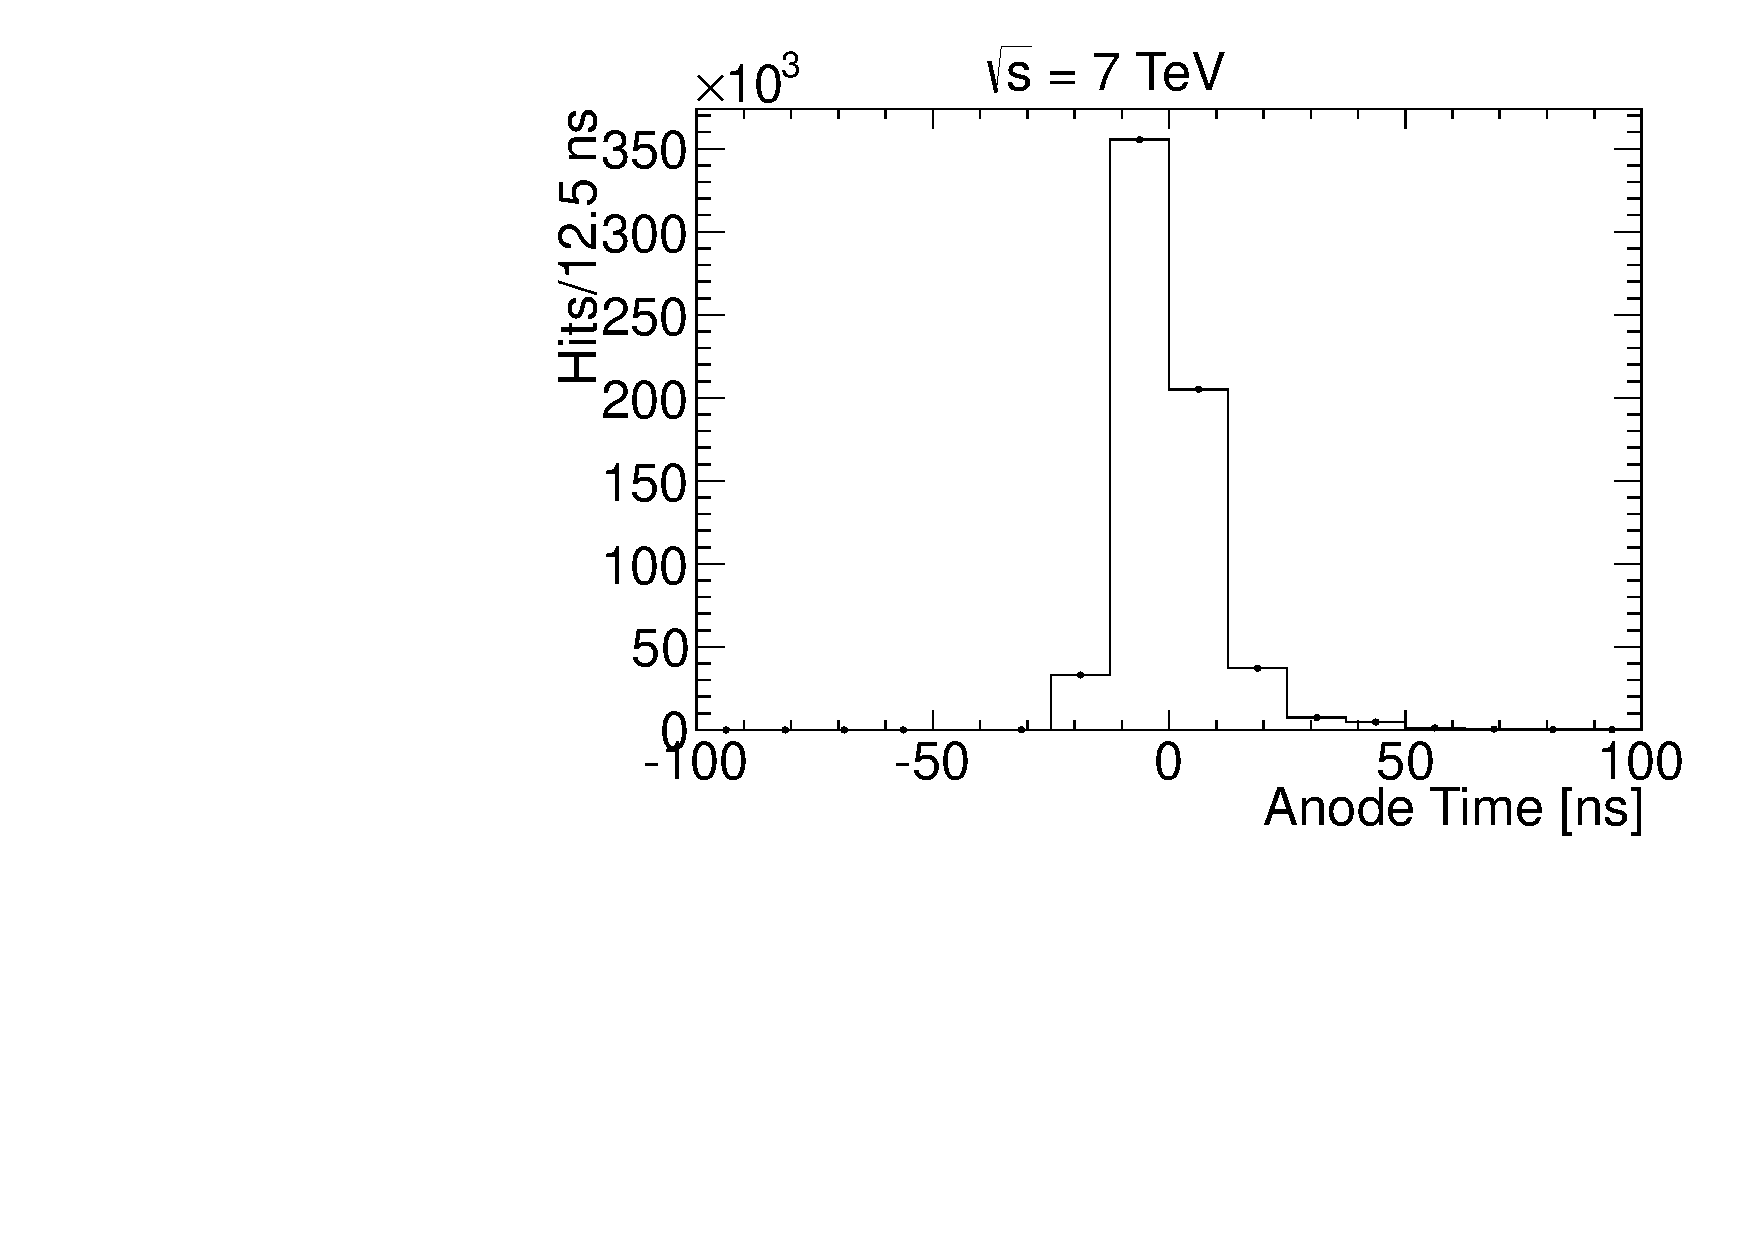
\includegraphics[clip=true, trim=0.0cm 0cm 2.0cm 0cm, width=0.44\textwidth]{figures/timing/AnodeTime} \\
      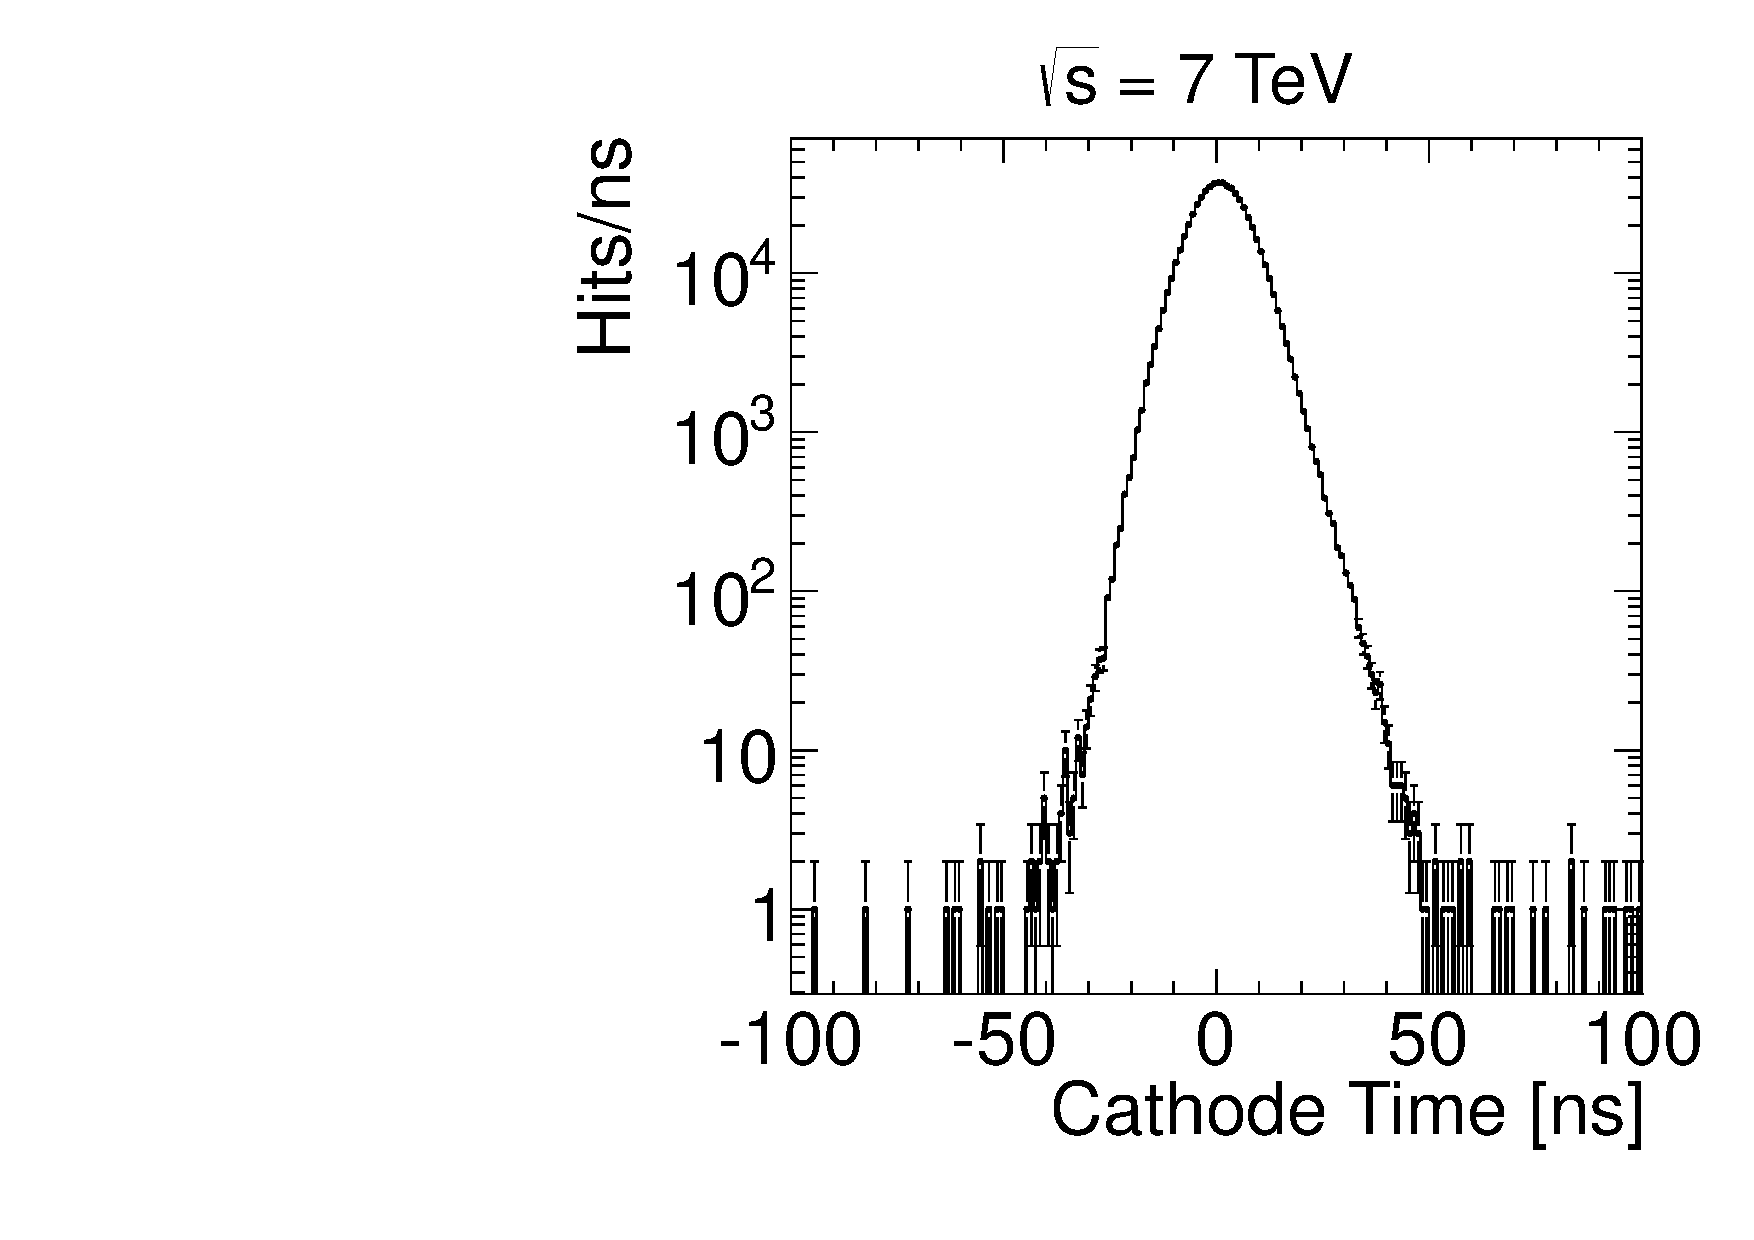
\includegraphics[clip=true, trim=0.0cm 0cm 2.0cm 0cm, width=0.44\textwidth]{figures/timing/CathodeTimeLog}
      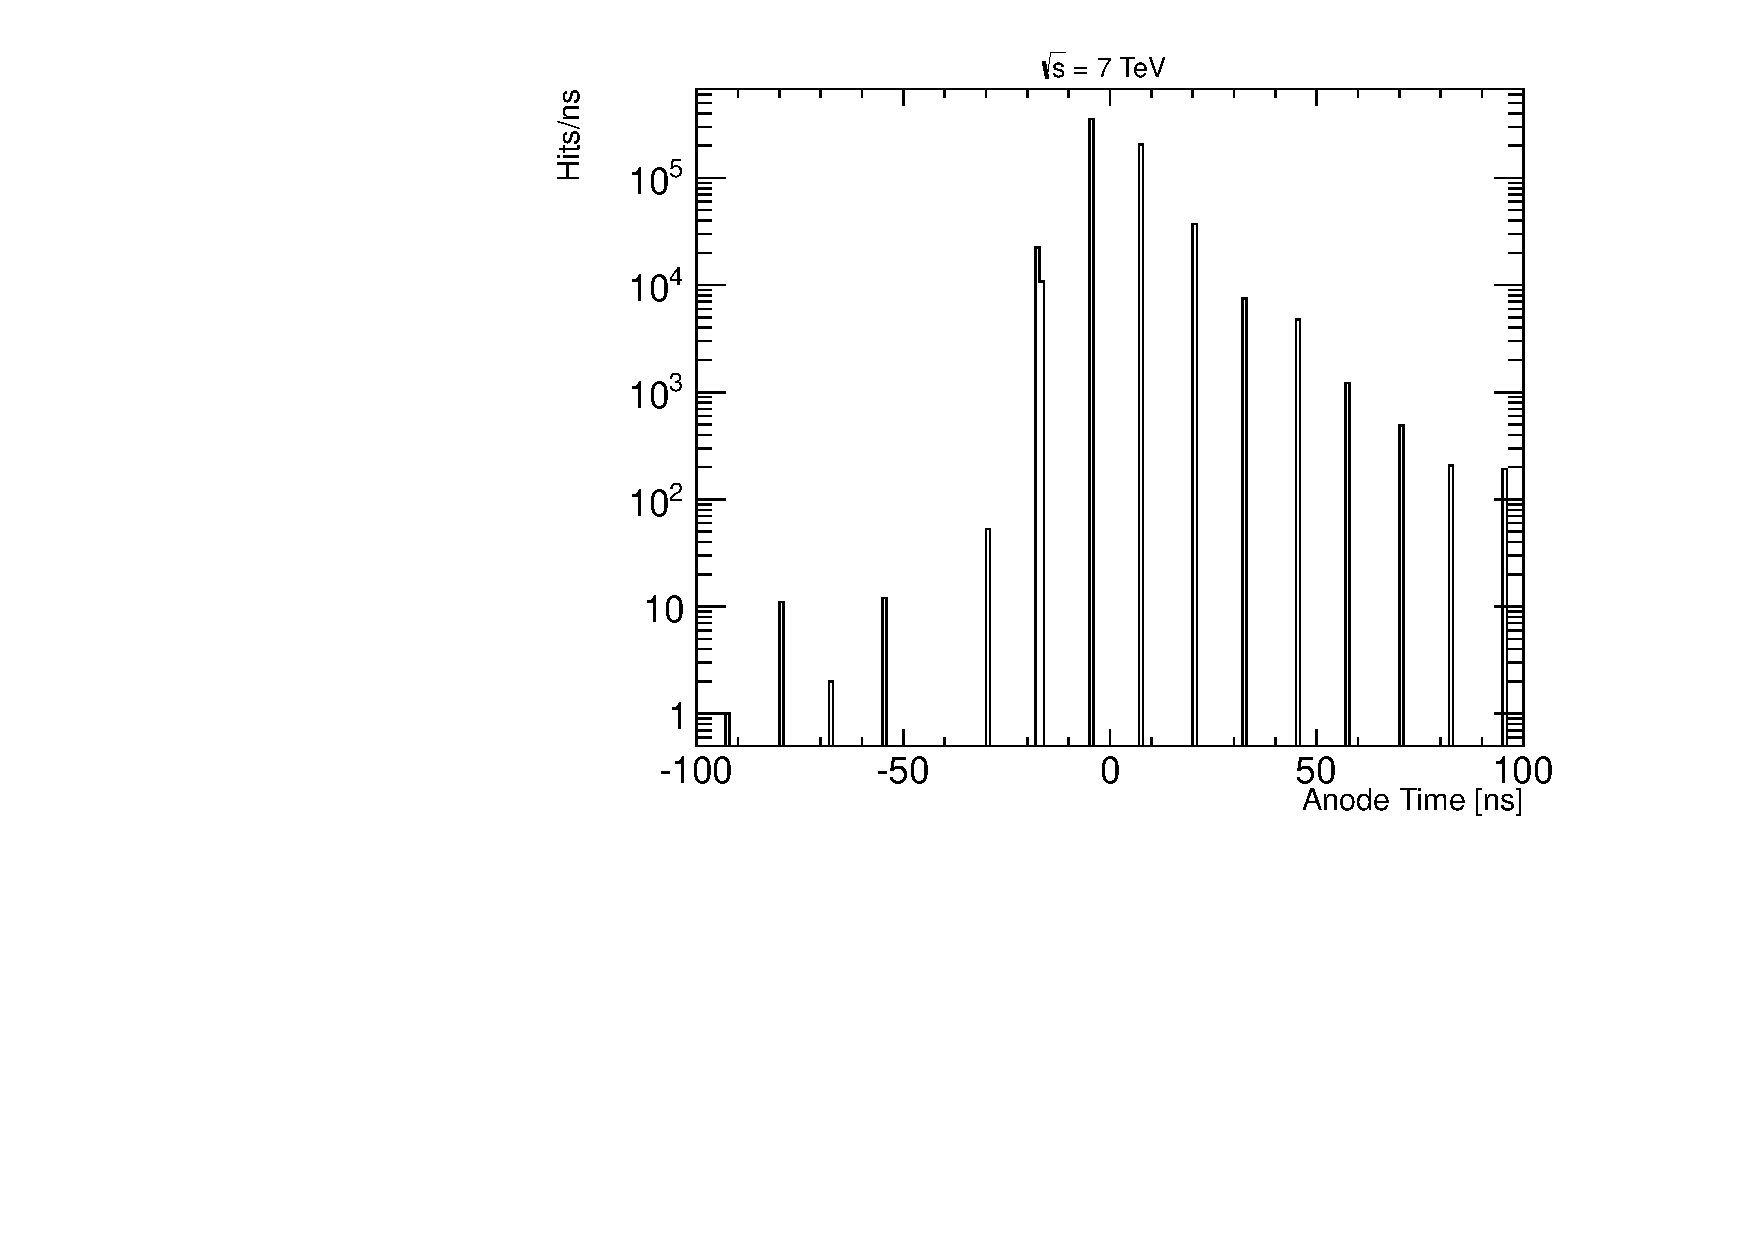
\includegraphics[clip=true, trim=0.0cm 0cm 2.0cm 0cm, width=0.44\textwidth]{figures/timing/AnodeTimeLog} \\
      \caption[Distribution of time of anode and cathode hits]
      {Left column: Distribution of cathode time of hits. Right column: Distribution of anode time of hits. Top row: Linear scale. Bottom row: Log scale.
	}
      \label{fig:hittime}
  \end{center}
\end{figure}

The anode and cathode hits in a chamber are used to reconstruct a segment which is meant to represent the passage of the particle through the chamber. A time is
associated with the segments by averaging the anode and cathode times associated with the segments. The times are weighted by one over their variance.
To remove the large tail in the anode time measurement,
a cleaning procedure is applied to the anode times to remove outlier hits. The procedure removes anode times more than three
sigma different from the average. The times of segments associated with high quality muons is shown in Fig.~\ref{fig:SegTimes}. The resolution on the segment times is 3.0ns.

\begin{figure}
  \begin{center}
      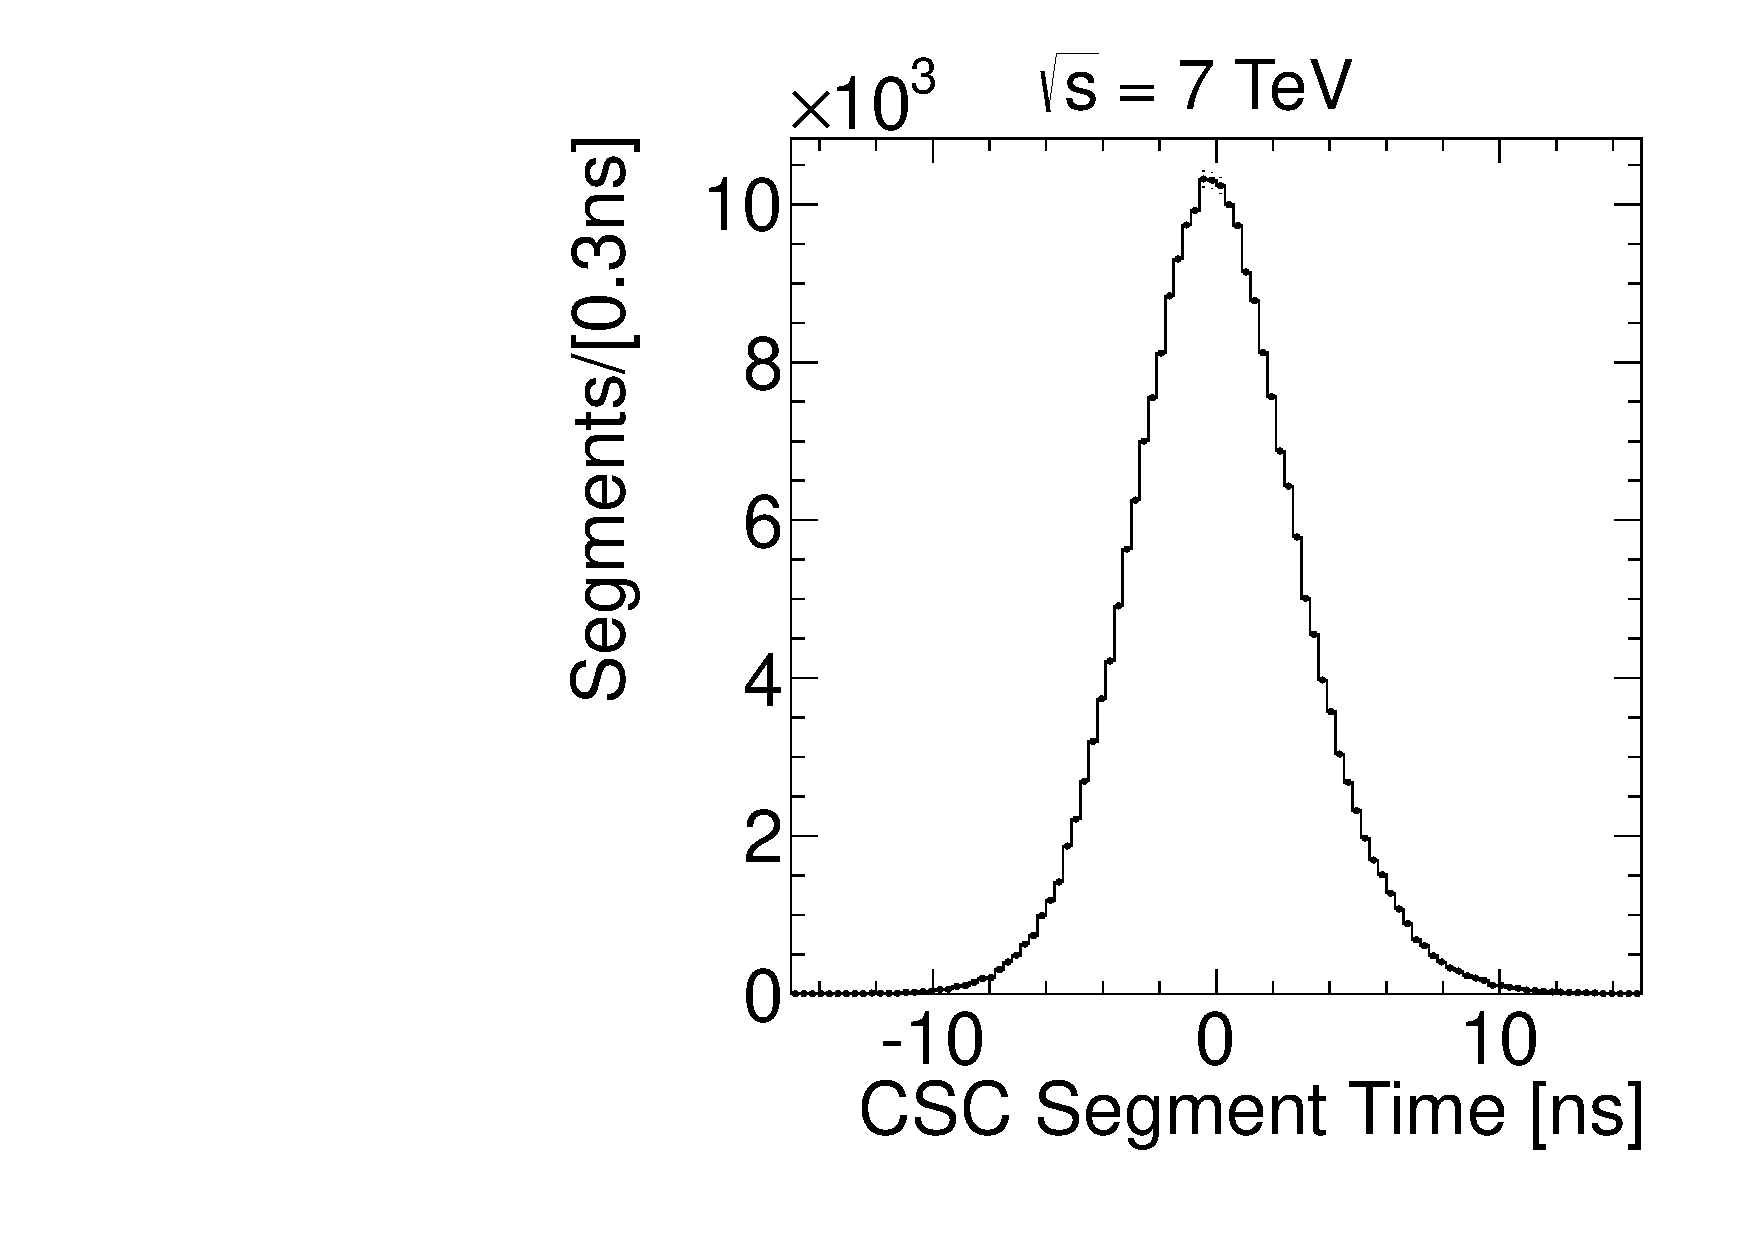
\includegraphics[width=0.44\textwidth]{figures/timing/StripAndWireSegmentTime}
      \caption[Distribution of times of segments associated with high quality muons]
      {Times of segments associated with high quality muons.
        }
      \label{fig:SegTimes}
  \end{center}
\end{figure}

\section{CSC Trigger Timing}

The CSCs are a key component of the L1 trigger system and it is important that they associate tracks in the system with the correct LHC bunch crossing window.
The CSCs build tracks for the L1 trigger with the CSC Track Finder (CSCTF) by combining track stubs coming from the CSC chambers. 
The stubs are associated with a particular bunch crossing window and
the track finder uses majority logic of the stubs used to build the track to associate the track with a bunch crossing window. In cases where there are an equal number
of stubs from different bunch crossing windows, say two track stubs coming from adjacent bunch crossing windows, the CSCTF preferentially selects the later bunch crossing window.

As mentioned in Section~\ref{sec:subsystems}, there are six layers of cathode strips and anode wires in a CSC chamber.
Electronics on the chamber collect hits from the cathode strips and anode wires and separately create trigger primitives called Cathode Local Charged Track (CLCT)
and Anode Local Charged Track (ALCT), respectively. The two separate trigger primitives are then combined to form a Local Charged Track (LCT). The trigger primitives
must be associated with events within three bunch crossing windows of one another to be combined.
The bunch crossing window that the LCT is associated with is set by the ALCT.

The timing of the ALCT is determined by the timing of the third anode hit, its first high bit, 
to arrive to the ALCT circuit board. A common offset per chamber can be applied to the
anode hits to give the best timing synchronization of the ALCTs. To determine the offset the arrival time of the anode hits is studied offline using hits from
high quality muons. The average time of the anode
hits can be correlated with the probability for a chamber to produce an ALCT in the bunch crossing window before it should (pretrigger) and after it should (posttrigger).
The offsets for each chamber can be tuned to give an expected pretrigger and posttrigger probability.

However, the CSCTF logic means that simply setting the offset to give an equal probability to pretrigger and posttrigger is not optimal. This can be seen by looking at
the case where the CSCTF only receives two track stubs, this is also the case where the CSC online timing is most important. If the CSCTF receives one LCT in the bunch
crossing window before the collision and one in the correct bunch crossing window, it will preferentially choose the later LCT and associate the combined track with the correct
bunch crossing window.  In order to pretrigger the readout of the event more than one LCT must arrive early.
On the other hand, if it recieves one LCT in the correct bunch crossing window and one in the proceeding bunch crossing window, the track will be associated with the
bunch crossing window following the collision. Thus, the probability to pretrigger the event can be written as $P_{LCTPre}^2$ while the posttrigger probability can be written as
$2 \times P_{LCTPost} - P_{LCTPost}^2$. 

Figure~\ref{fig:AnodevsprePost} shows the probabilities to pretrigger and posttrigger both at the chamber level and the expected probability at the CSCTF versus
the average anode time of a chamber. The chambers are split into three categories depending on which station and ring they belong to. One category is chambers in the
first ring and station, another the chambers in the first ring not in the first station, and the last those not in the first ring. The design of these chambers are all
slightly different so it is allowed for them to have different optimal times.

\begin{figure}
  \begin{center}
      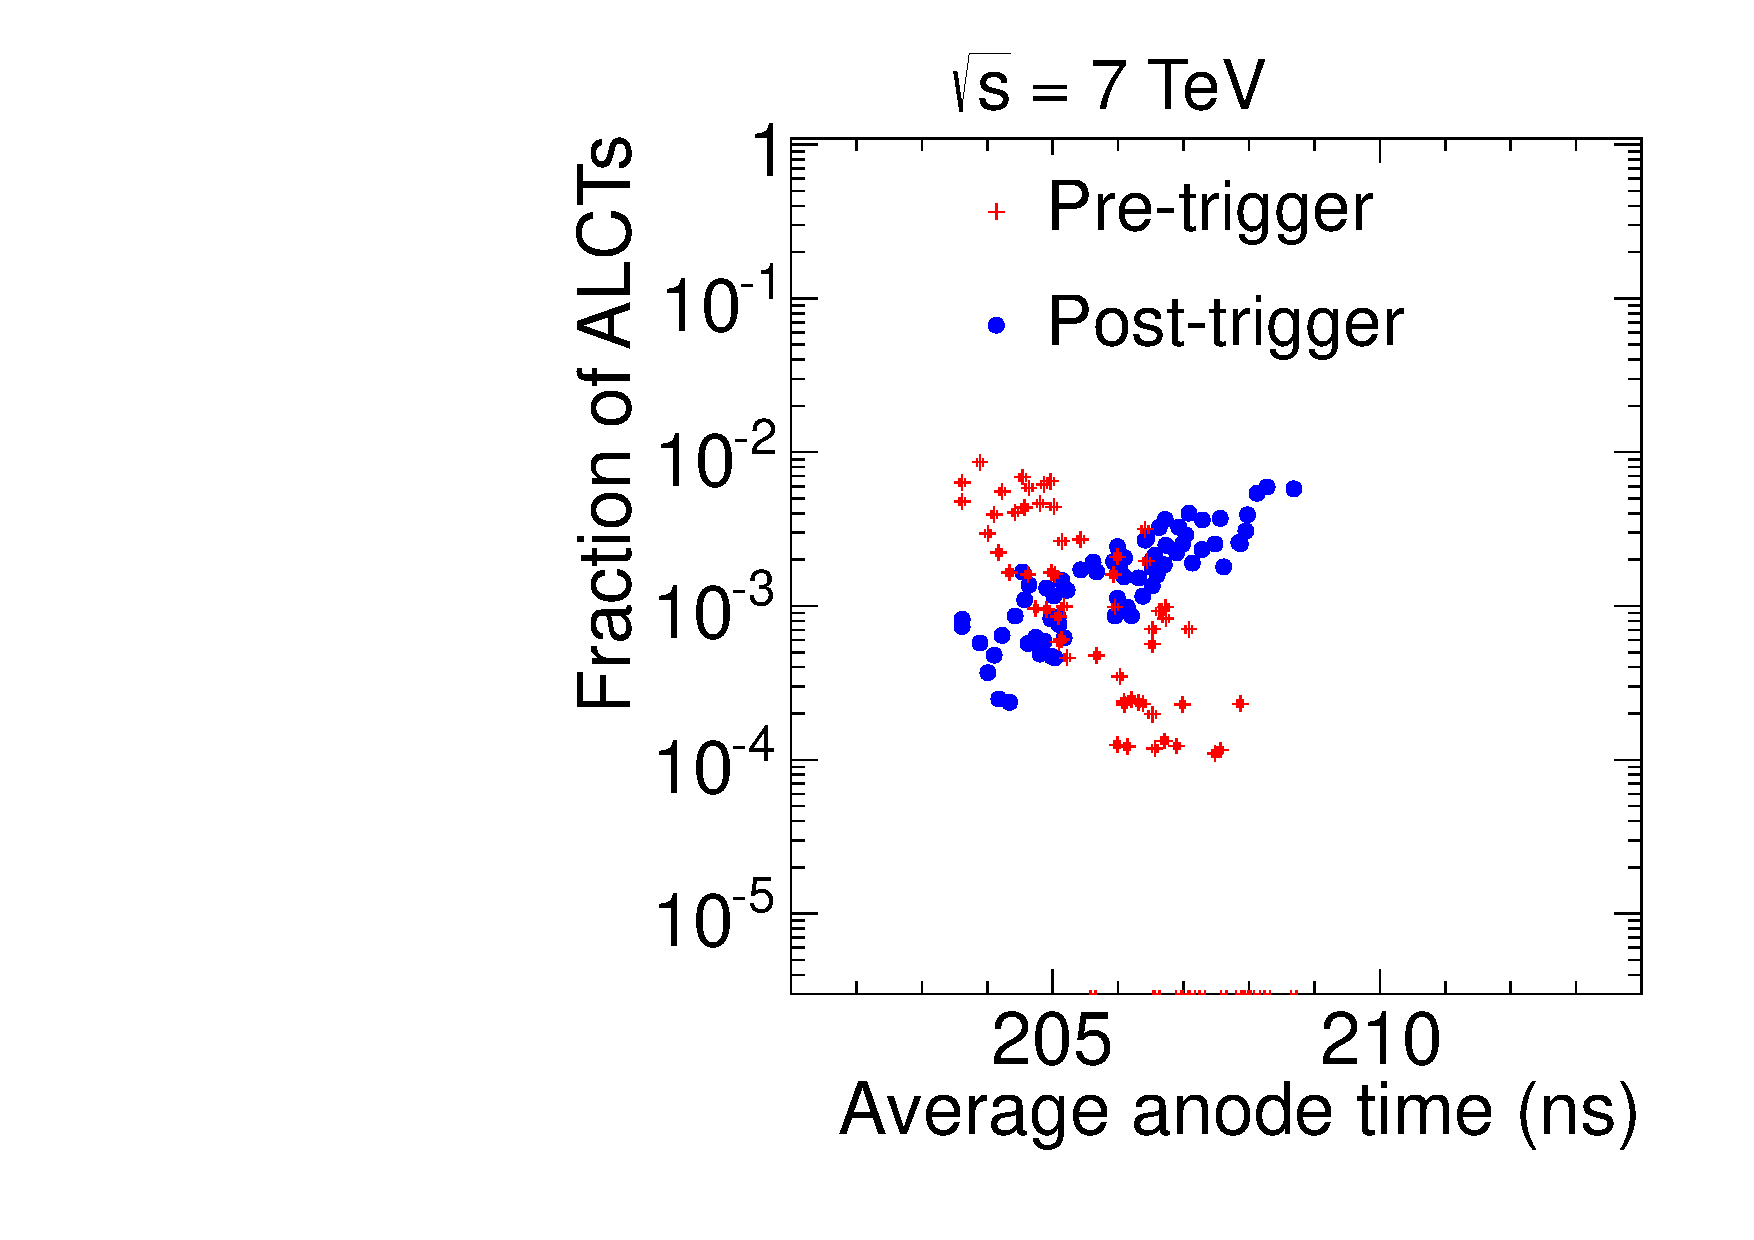
\includegraphics[clip=true, trim=0.0cm 0cm 3.0cm 0cm, width=0.44\textwidth]{figures/timing/ME11_Anode_vs_all3}
      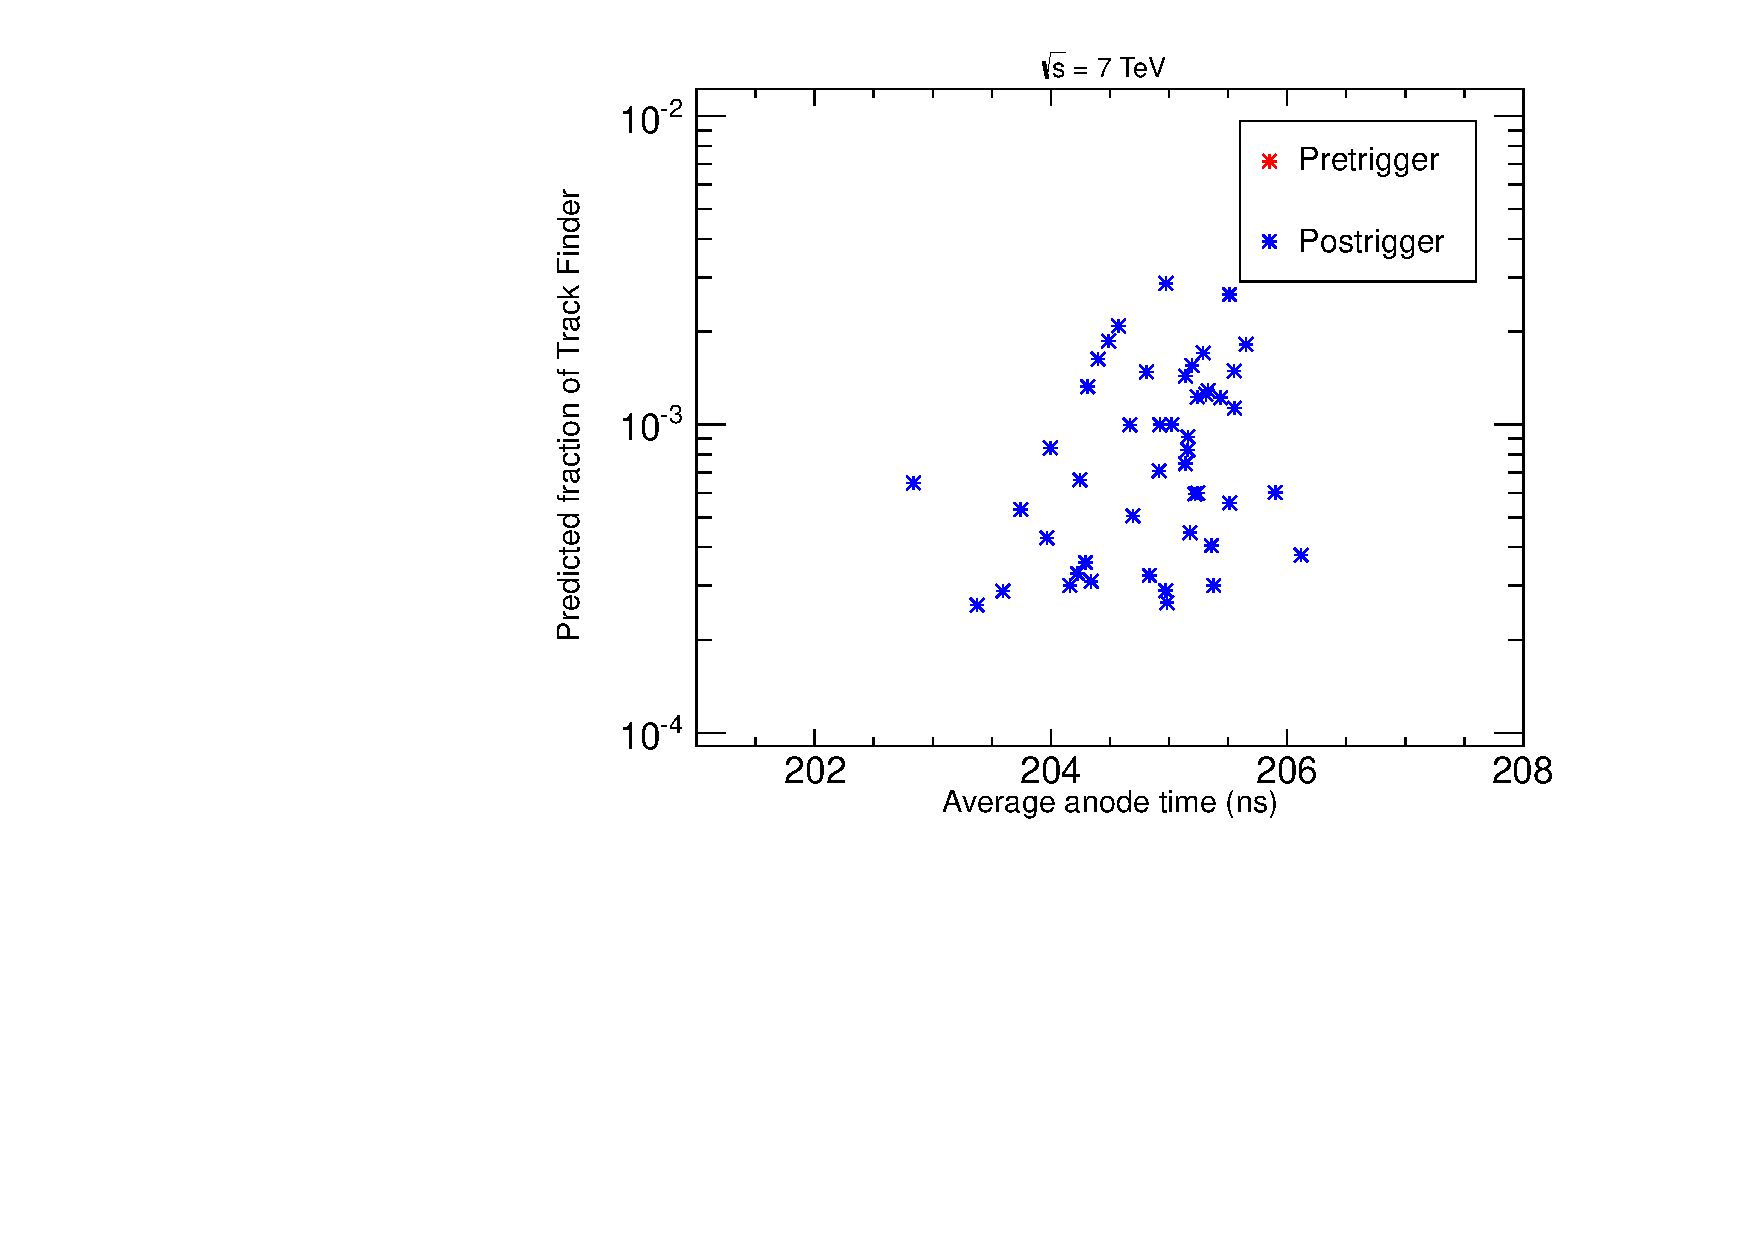
\includegraphics[clip=true, trim=0.0cm 0cm 3.0cm 0cm, width=0.44\textwidth]{figures/timing/ME11_Anode_vs_TF_all} \\
      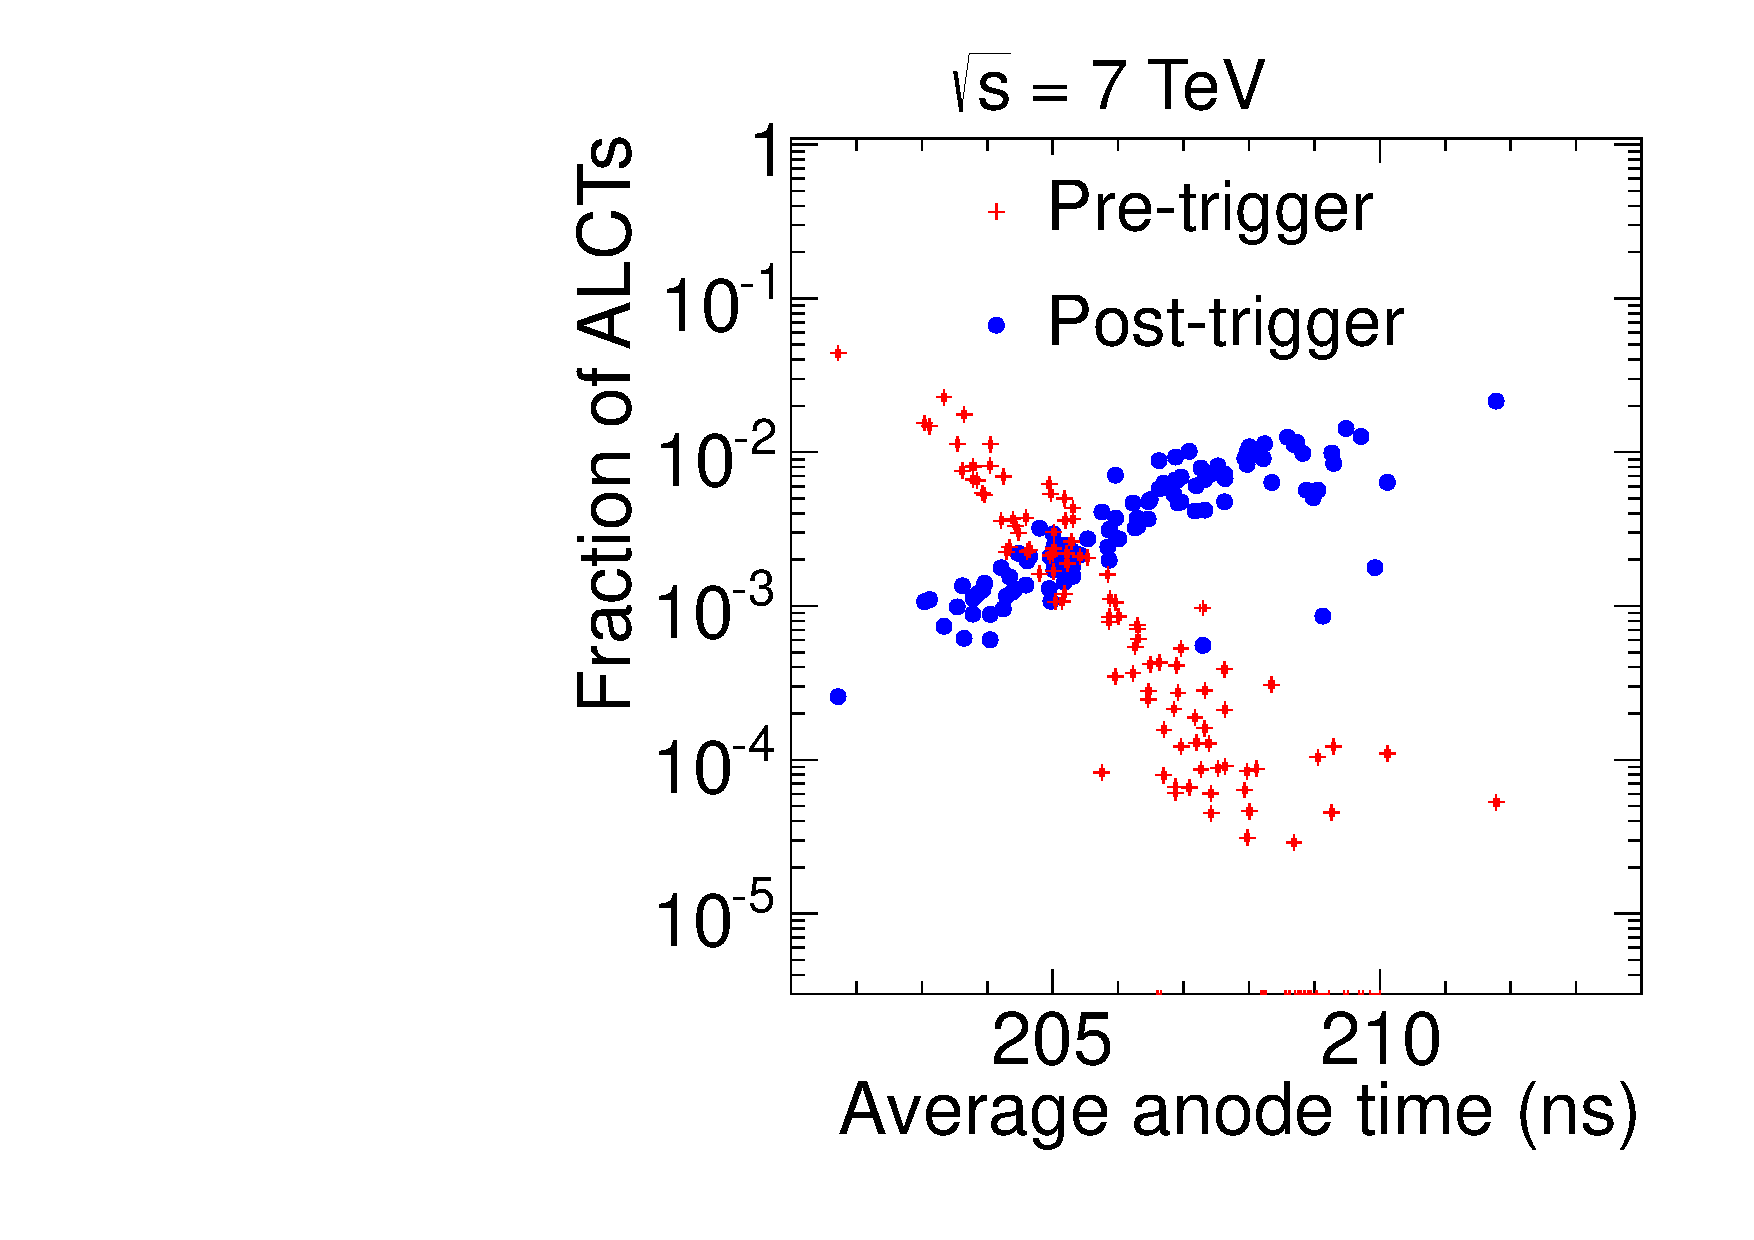
\includegraphics[clip=true, trim=0.0cm 0cm 3.0cm 0cm, width=0.44\textwidth]{figures/timing/Ring1_not11_Anode_vs_all3}
      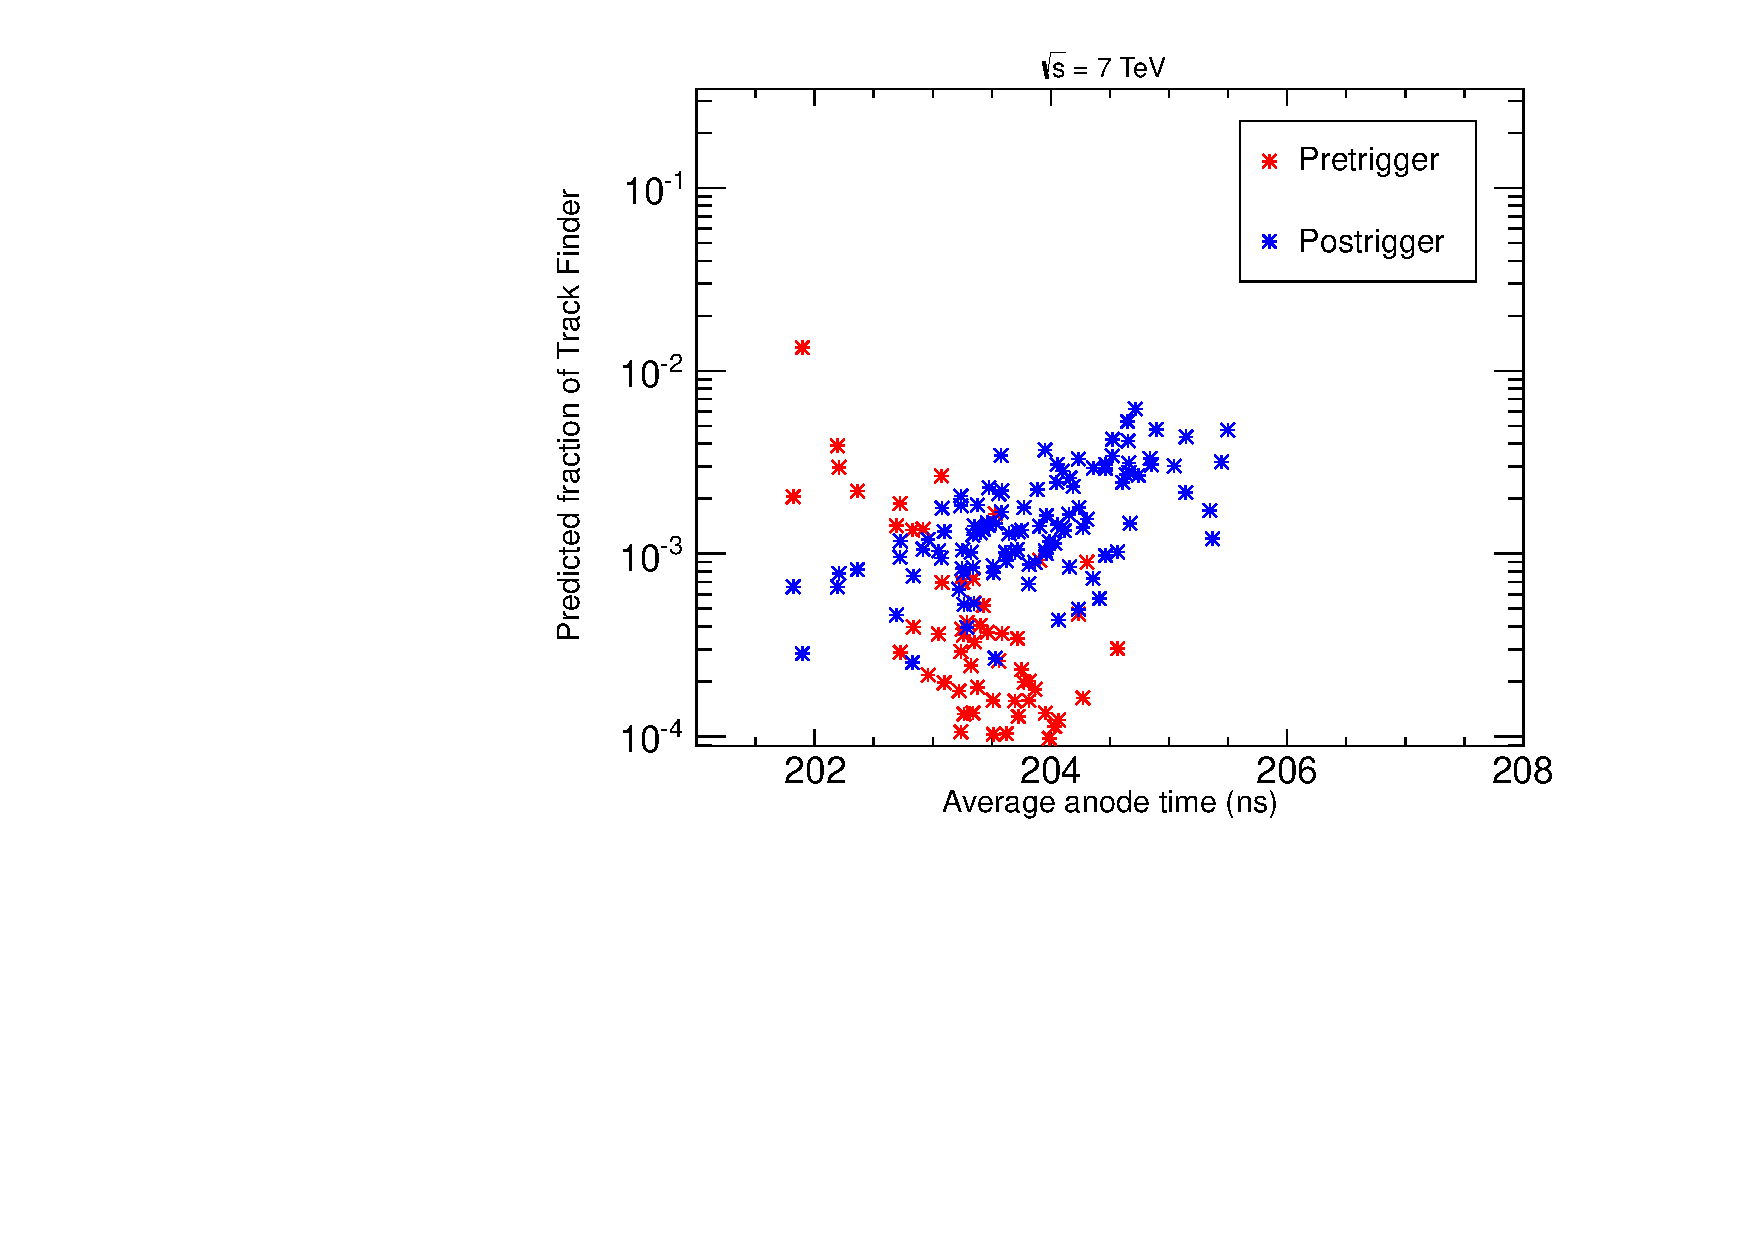
\includegraphics[clip=true, trim=0.0cm 0cm 3.0cm 0cm, width=0.44\textwidth]{figures/timing/Ring1_not11_Anode_vs_TF_all} \\
      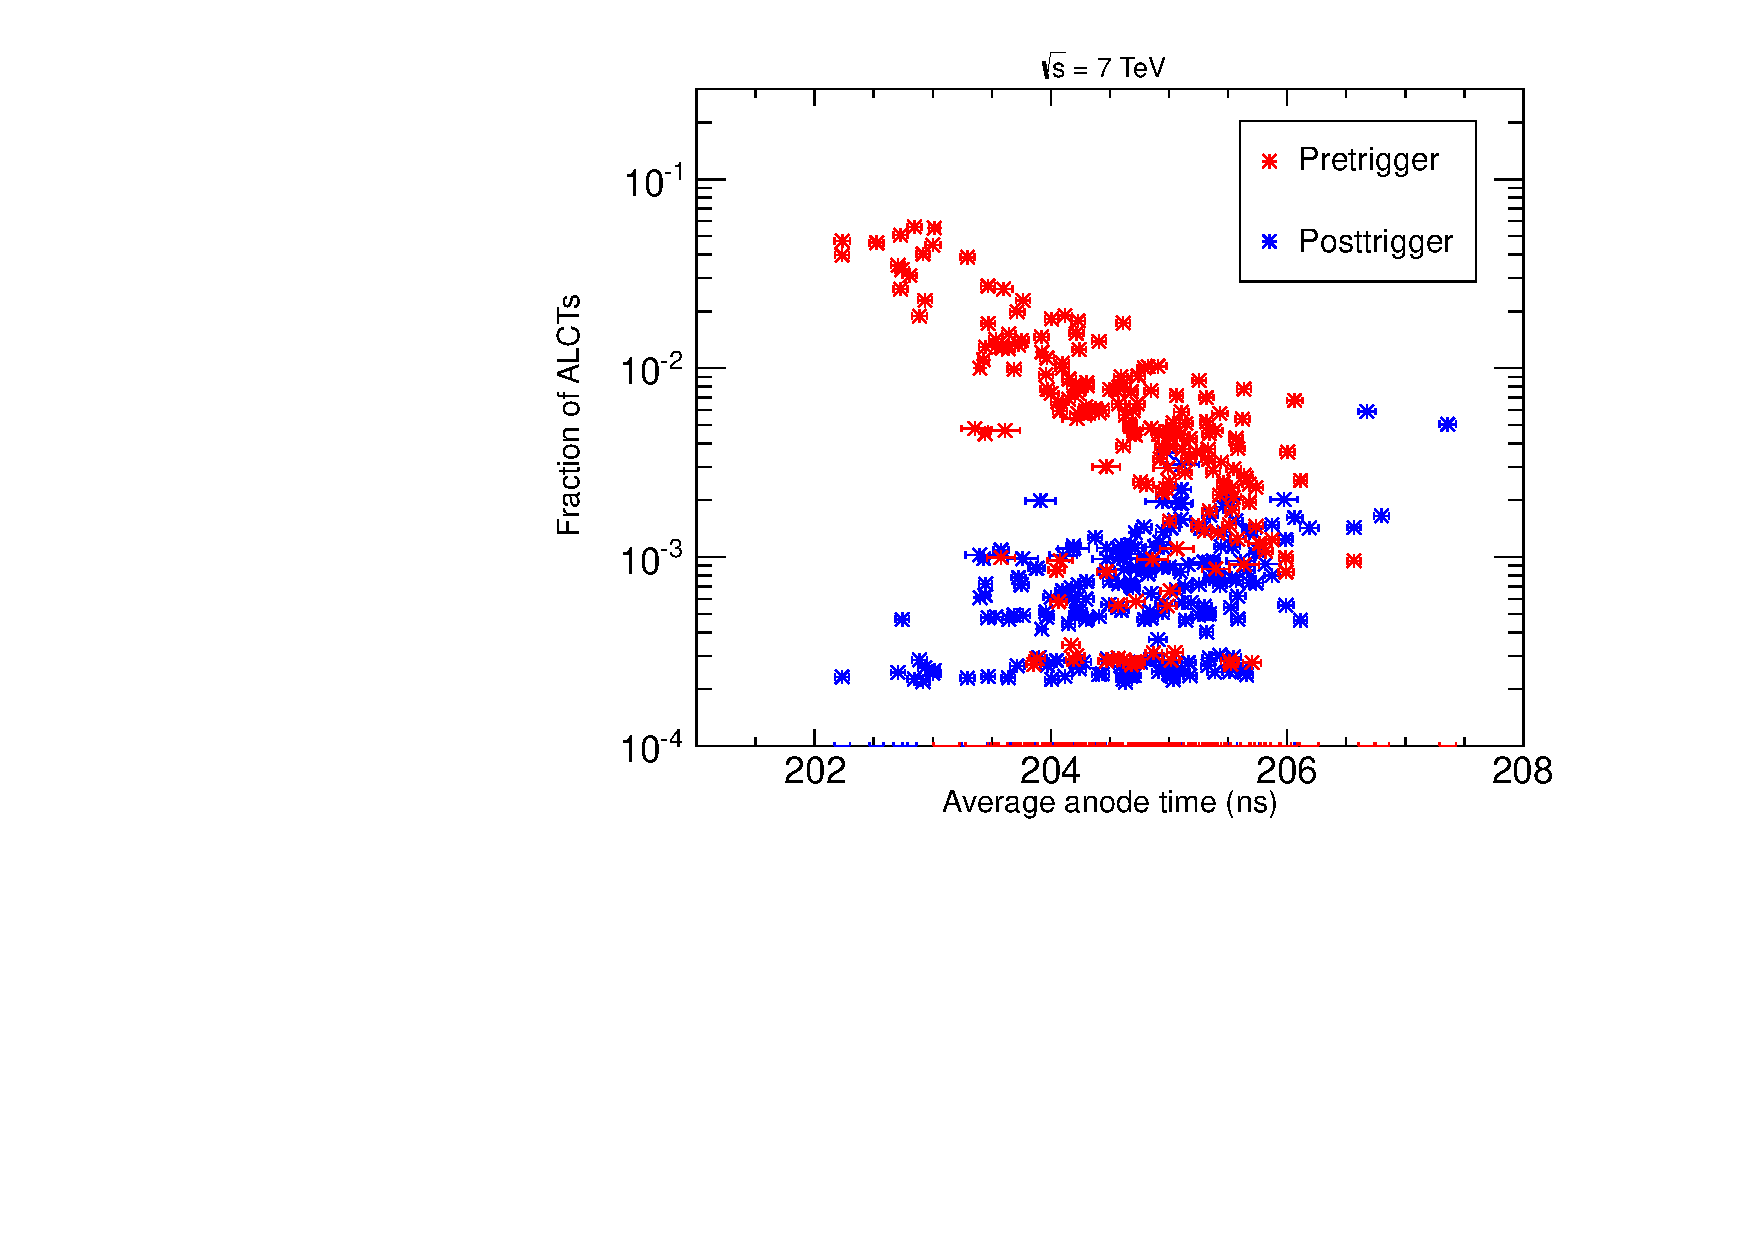
\includegraphics[clip=true, trim=0.0cm 0cm 3.0cm 0cm, width=0.44\textwidth]{figures/timing/Ring2_Anode_vs_all3}
      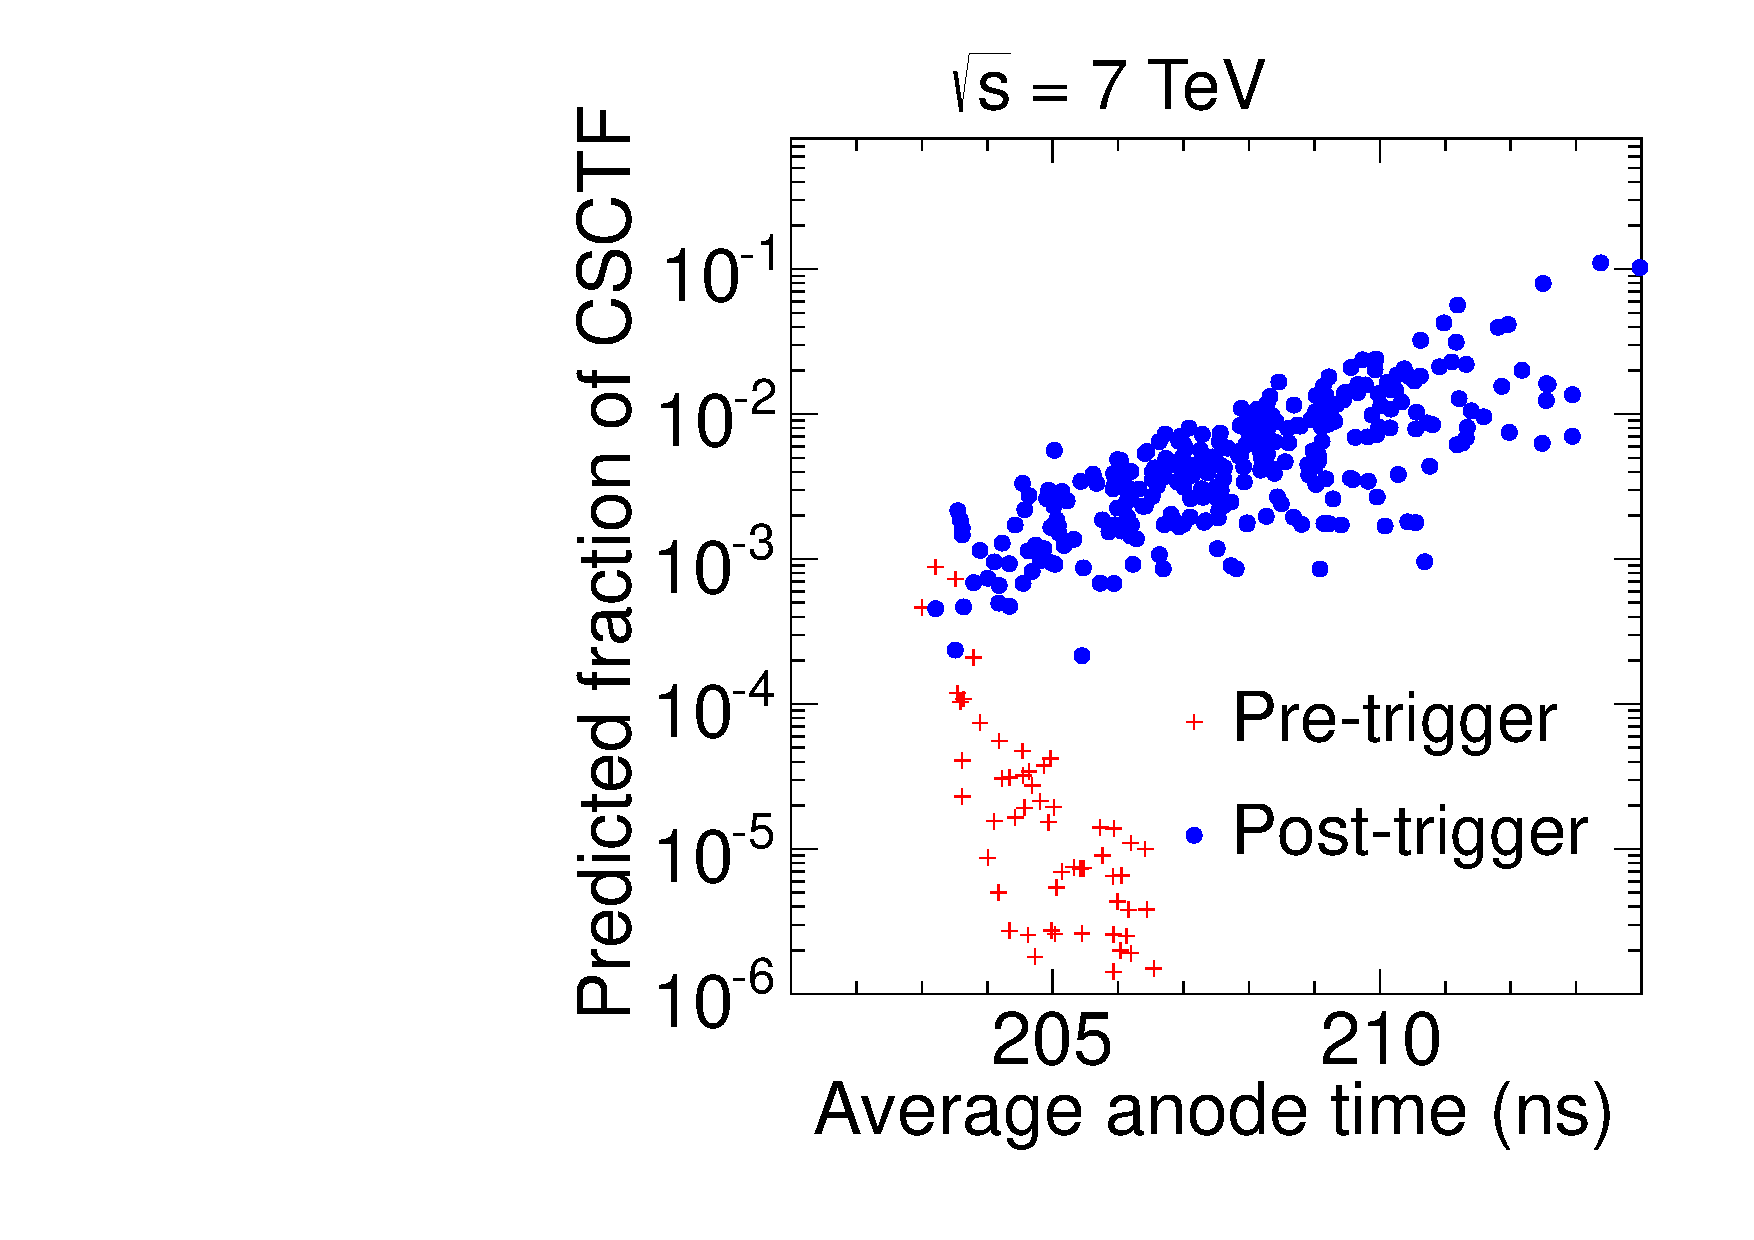
\includegraphics[clip=true, trim=0.0cm 0cm 3.0cm 0cm, width=0.44\textwidth]{figures/timing/Ring2_Anode_vs_TF_all} \\
      \caption[CSC pretriggering and posttriggering versus average anode time for LCTs and expected behavior at CSCTF]
      {Pretriggering and posttriggering versus average anode time. Left column shows the pretriggering and posttriggering for LCTs.
Right column shows what would be expected at the CSCTF. Top row for chambers in the innermost ring and station. Middle row is for all other chambers in the innermost ring.
Last row is for all other chambers.
        }
      \label{fig:AnodevsprePost}
  \end{center}
\end{figure}

From these plots an optimal value of 204ns is chosen for the chambers in the first ring not in the first station and 205ns for all other chambers.
The plot of the pretriggering and posttriggering in the track finder somewhat implies an earlier optimal but these are not used for two reasons.
The first is that pretriggering grows as the square of the pretriggering probability and since, as described below, the offsets can not be set exactly, chambers
that are slightly below optimal could lead to significant pretriggering in those chambers. Second, pretriggering prevents the readout of the collision event even by
another portion of the detector, CMS can not readout two consecutive events, while posttriggering does not have this issue. For these reasons slightly later times
that still have very low posttriggering are used.

The offsets can be moved in roughly 2 ns steps in the chamber firmware with the actual number possibly being different chamber to chamber. Shifting the offsets is a
somewhat complicated procedure and carries the risk of accidentally shifting the timing of a chamber by a large amount. Thus, the offsets are changed only
when deemed necessary, numerous iterations to get a perfect synchronization are not done. The synchronization with respect to the optimal values for all chambers
is shown in Fig.~\ref{fig:average_anodes}, most of the chambers are within one ns of the optimal time with none more than three ns off.

\begin{figure}
  \begin{center}
      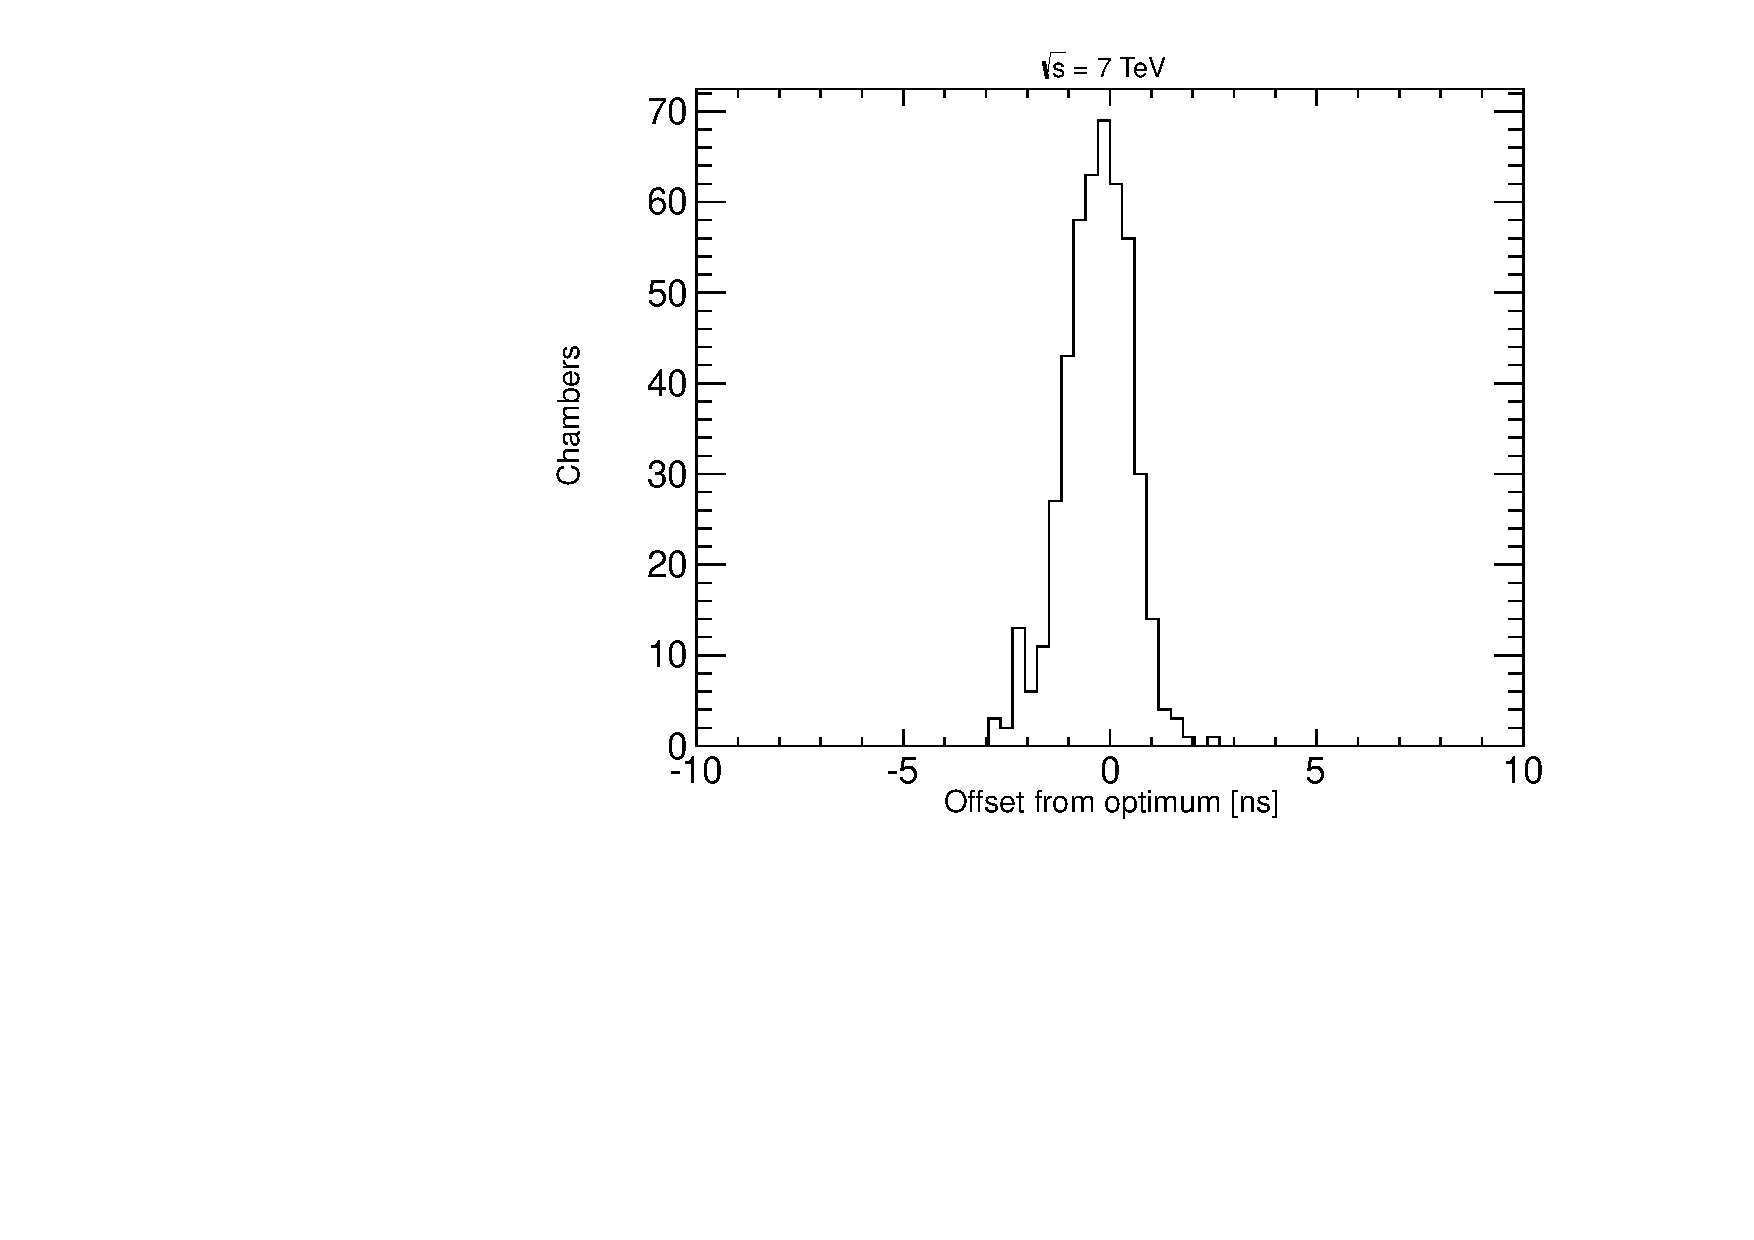
\includegraphics[clip=true, trim=0.0cm 0cm 3.0cm 0cm, width=0.44\textwidth]{figures/timing/average_anodes}
      \caption[Average anode time of chambers relative to optimal values.]
      {Average anode time of chambers relative to optimal values.
        }
      \label{fig:average_anodes}
  \end{center}
\end{figure}

After this synchronization procedure is performed the timing of the LCTs is very good. This can be seen in Fig.~\ref{fig:ALCTBX} which shows the bunch crossing window
assigned to LCT matched to high quality muons. The distribution is purposefully made asymmetric to account for the CSCTF logic used further downstream.
The efficiency is 99\%, better than the 92\% design requirement.

\begin{figure}
  \begin{center}
      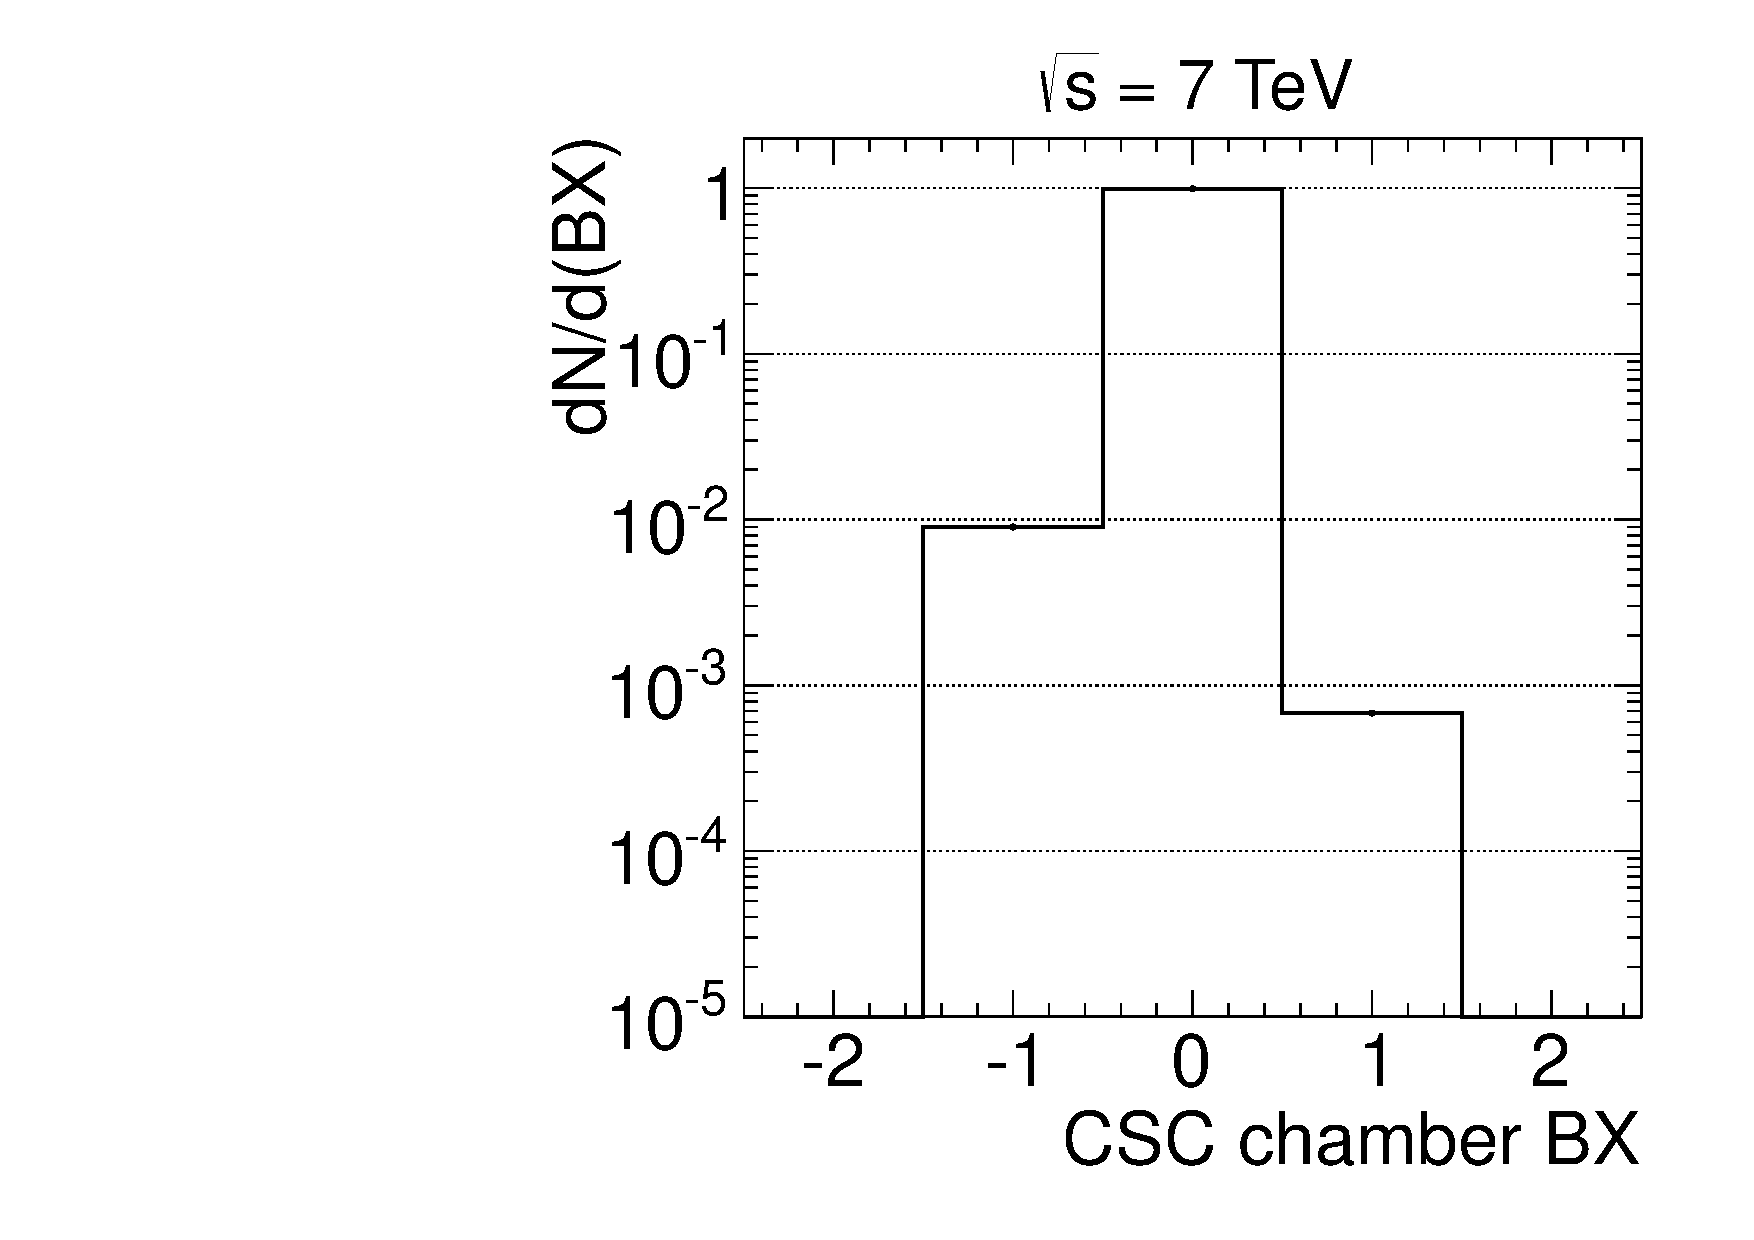
\includegraphics[clip=true, width=0.44\textwidth]{figures/timing/ALCT_Bx}
      \caption[Fraction of LCTs versus LCT bunch crossing window assignment relative to collision event]
      {Fraction of LCTs versus LCT bunch cross assignment relative to collision event
        }
      \label{fig:ALCTBX}
  \end{center}
\end{figure}

\section{Muon Track Timing}

Tracks, meant to represent muons or other particles passing through the detector, are built in the muon system connecting together the hits in the different chambers of
the CSCs, DTs, and RPCs. Numerous different timing quantities about the track are calculated under three different assumptions on how the particle
travels between the interaction point and the muon system. Only time measurements from the CSCs and DTs are used to calculate the timing quantities.

A particle of speed, v, travelling from the interaction point, will arrive at a location d in the muon system at
%~\ref{eq:speed}

\begin{equation}
t = d/v + t_0
\label{eq:speed}
\end{equation}

where $t_0$ is an overall offset. When the local timing variables were defined, they were calibrated such that a speed of light, c, particle would have an average time
of zero. Thus $d/c$ has already been subtracted from the times so the same quantity must be subtracted from the right hand side of~\ref{eq:speed}.
Additionally it is easier to work with \invbeta\ ($\equiv{c/v}$) instead of v. With these two ideas taken into mind Eq.~\ref{eq:speed} now becomes
\begin{equation}
\begin{split}
t &= d/v - d/c + t_0 \\
t &= d \times \beta^{-1} / c - d/c + t_0 \\
t &= (d / c) \times (\beta^{-1} - 1) + t_0 \\
\end{split}
\label{eq:speedred}
\end{equation}

The three assumptions relate to how the \invbeta\ and $t_0$ parameters are fixed and produce three different variables. 
The formula has two pieces of input datum, time, t, and distance, d. The distance
from the interaction point to the hit location is known to a much better degree than the time of the hit so the uncertainty on the variables comes 
almost entirely from the time measurement.

The first variable is the speed of the particle assuming it left the origin at $t_0 = 0$ reducing Eq.~\ref{eq:speed} to $t = (d / c) \times (\beta^{-1} - 1)$ or simpler
$\beta^{-1} = tc/d + 1$. The measurement of \invbeta\ comes from averaging this quantity for all the
CSC and DT hits associated with the track weighted as one over their variance.
% in the same manner as was done to caluclate their segment times.
Outlier hits from anode hits are again cleaned in the same manner as per the segment times. The weighting by one over variance and 
outlier cleaning is performed for all three measurements.

The motivation for using \invbeta\ now becomes clear, the \invbeta\ measurement
is linear with t, the source of the largest uncertainty. This means that \invbeta\ will have a much more normal shape than $\beta$ which would be skewed.
An important point here is that the distribution will be close to symmetrical for speed of light muons coming from the LHC.

The uncertainty on \invbeta\ can be calculated according to the formula
\begin{equation}
 \sigma_{1/\beta} = \sqrt{\sum_{i=1}^N \frac{(1/\beta_i - \overline{1/\beta})^2 \times w_{i}}{N-1}},
 \label{betaerr}
\end{equation}
where $\overline{1/\beta}$ is the average \invbeta\ of the track, $w_{i}$ is the weight of the ith hit, and N is the number of measurements associated with the track.

The speed of the particle is very useful in separating standard model muons from HSCP produced in new physics as is shown in Section~\ref{sec:search}.
Figure~\ref{fig:invbeta} shows the \invbeta\ measurement and its uncertainty for: data, completely dominated by collision muons; 
muons from the simulated Drell-Yan production of Z bosons and photons; cosmic ray muons, the sample is defined in~\ref{sec:search};
and HSCPs, again the sample is defined in~\ref{sec:search}. It can be seen that the data is strongly peaked at one, the cosmic ray muons are roughly flat, while
the HSCP have \invbeta\ greater than one, indicating they are traveling slowly.

\begin{figure}
  \begin{center}
      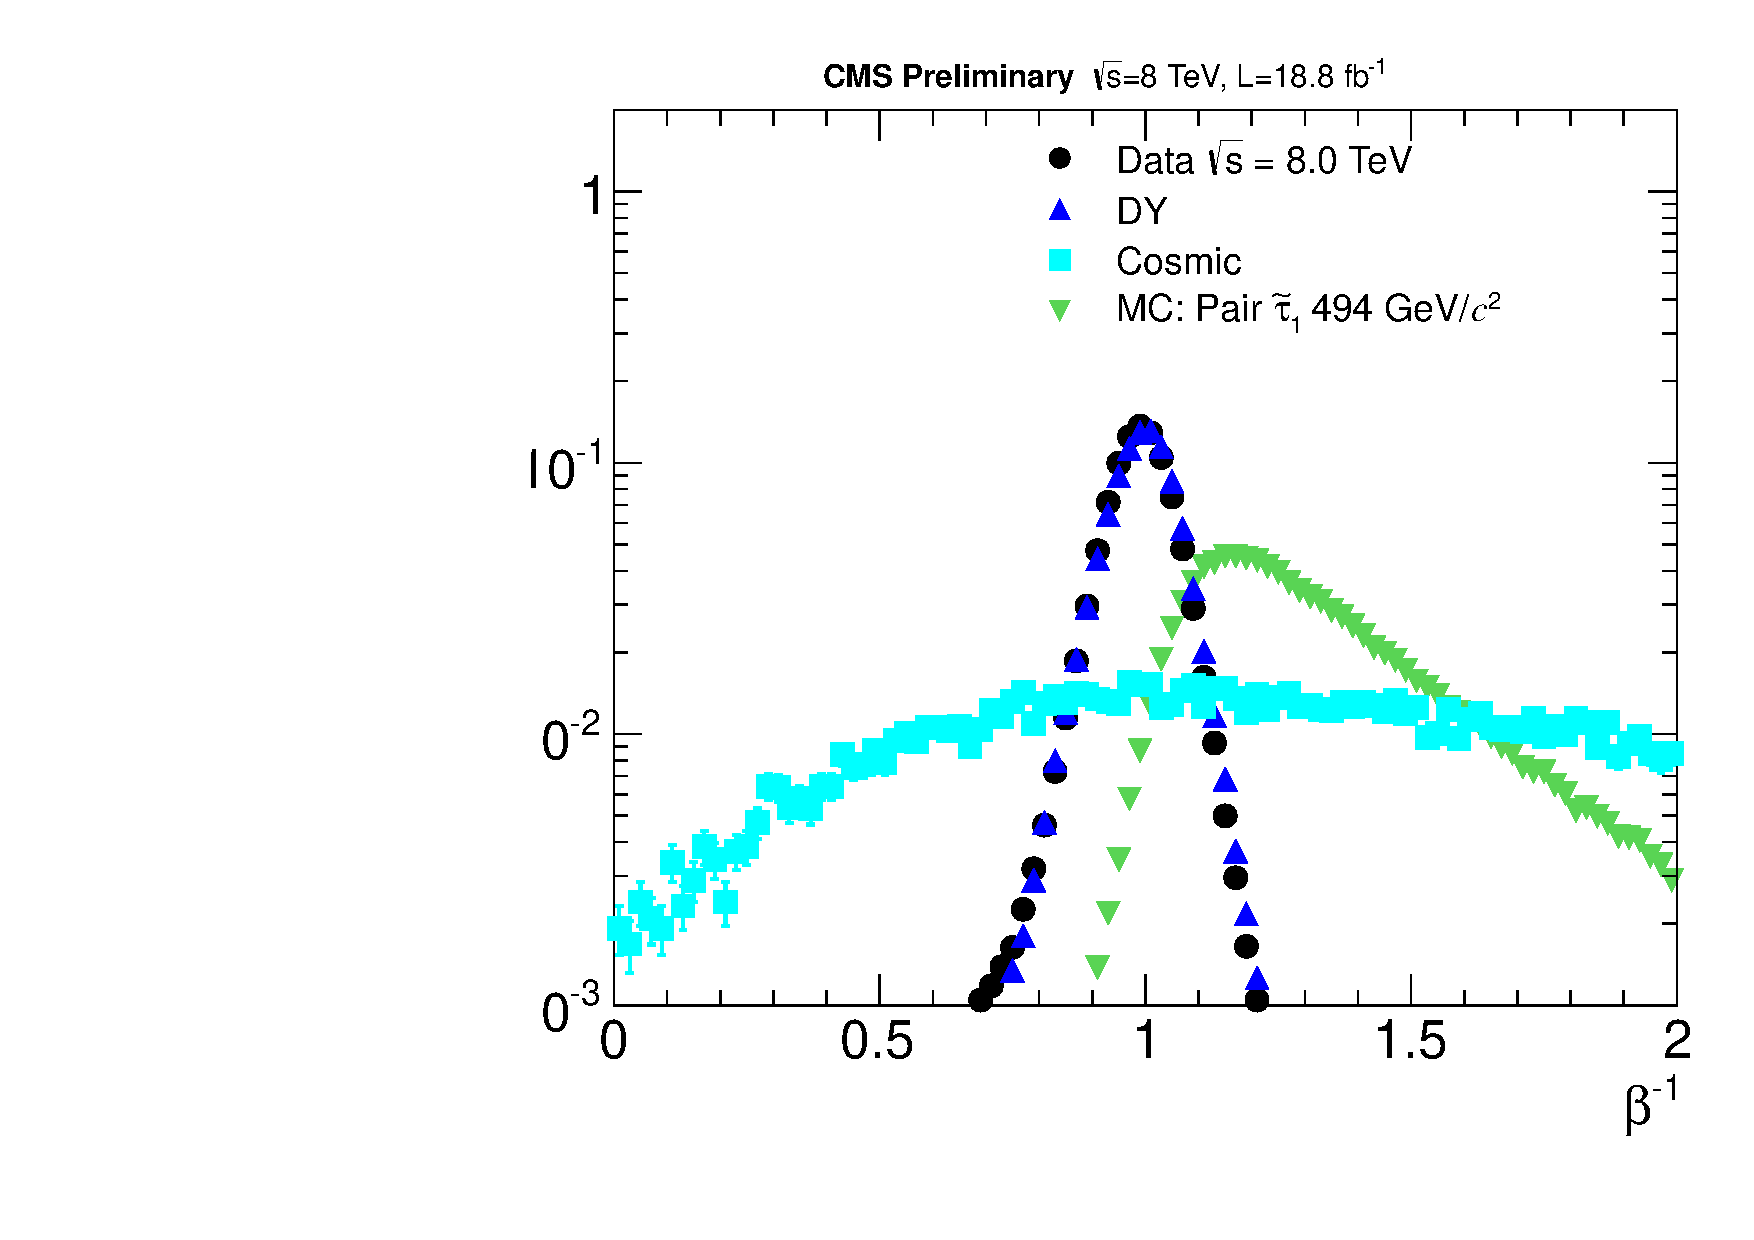
\includegraphics[width=0.44\textwidth]{figures/timing/TOF}
      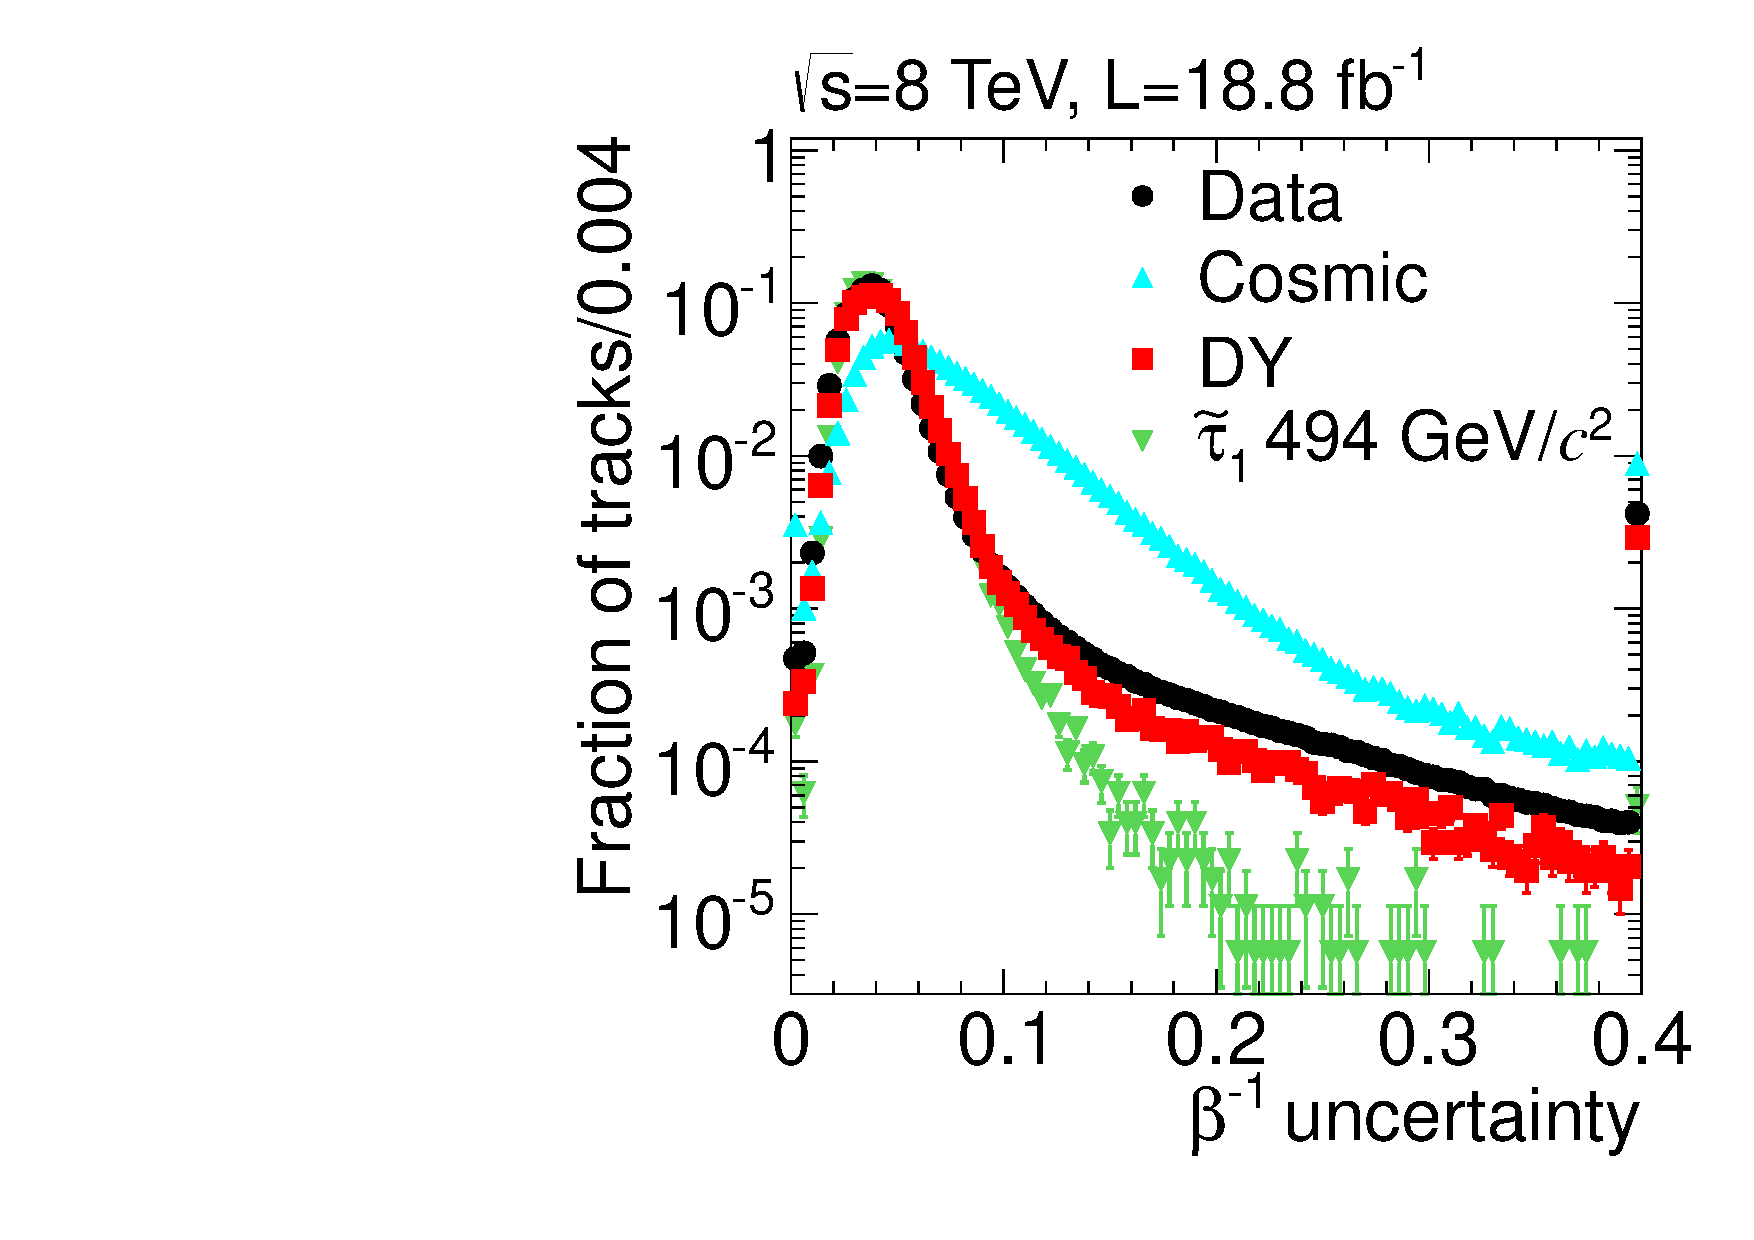
\includegraphics[width=0.44\textwidth]{figures/timing/TOFErr} \\
      \caption[Distribution of \invbeta\ and the uncertainty on \invbeta]
      {Distribution of \invbeta\ and the uncertainty on \invbeta\ for data,
simulated Drell-Yan production of photons and Z boson decaying to muons (DY), muons from cosmic rays, and simulated HSCPs
        }
      \label{fig:invbeta}
  \end{center}
\end{figure}


The next variable, time at vertex, is the estimated time the particle 
left the interaction point assuming it traveled at the speed of light.
This means setting \invbeta\ to be one in~\ref{eq:speed} reducing the equation to simply $t = t_0$. 
For muons with at least a modest amount of $p_T$ that are produced in a collision in the triggered bunch crossing window this assumption is valid and thus the
value should be centered at zero. Figure~\ref{fig:vertextime} shows the time at vertex for the same three samples as in~\ref{fig:invbeta}.

\begin{figure}
  \begin{center}
      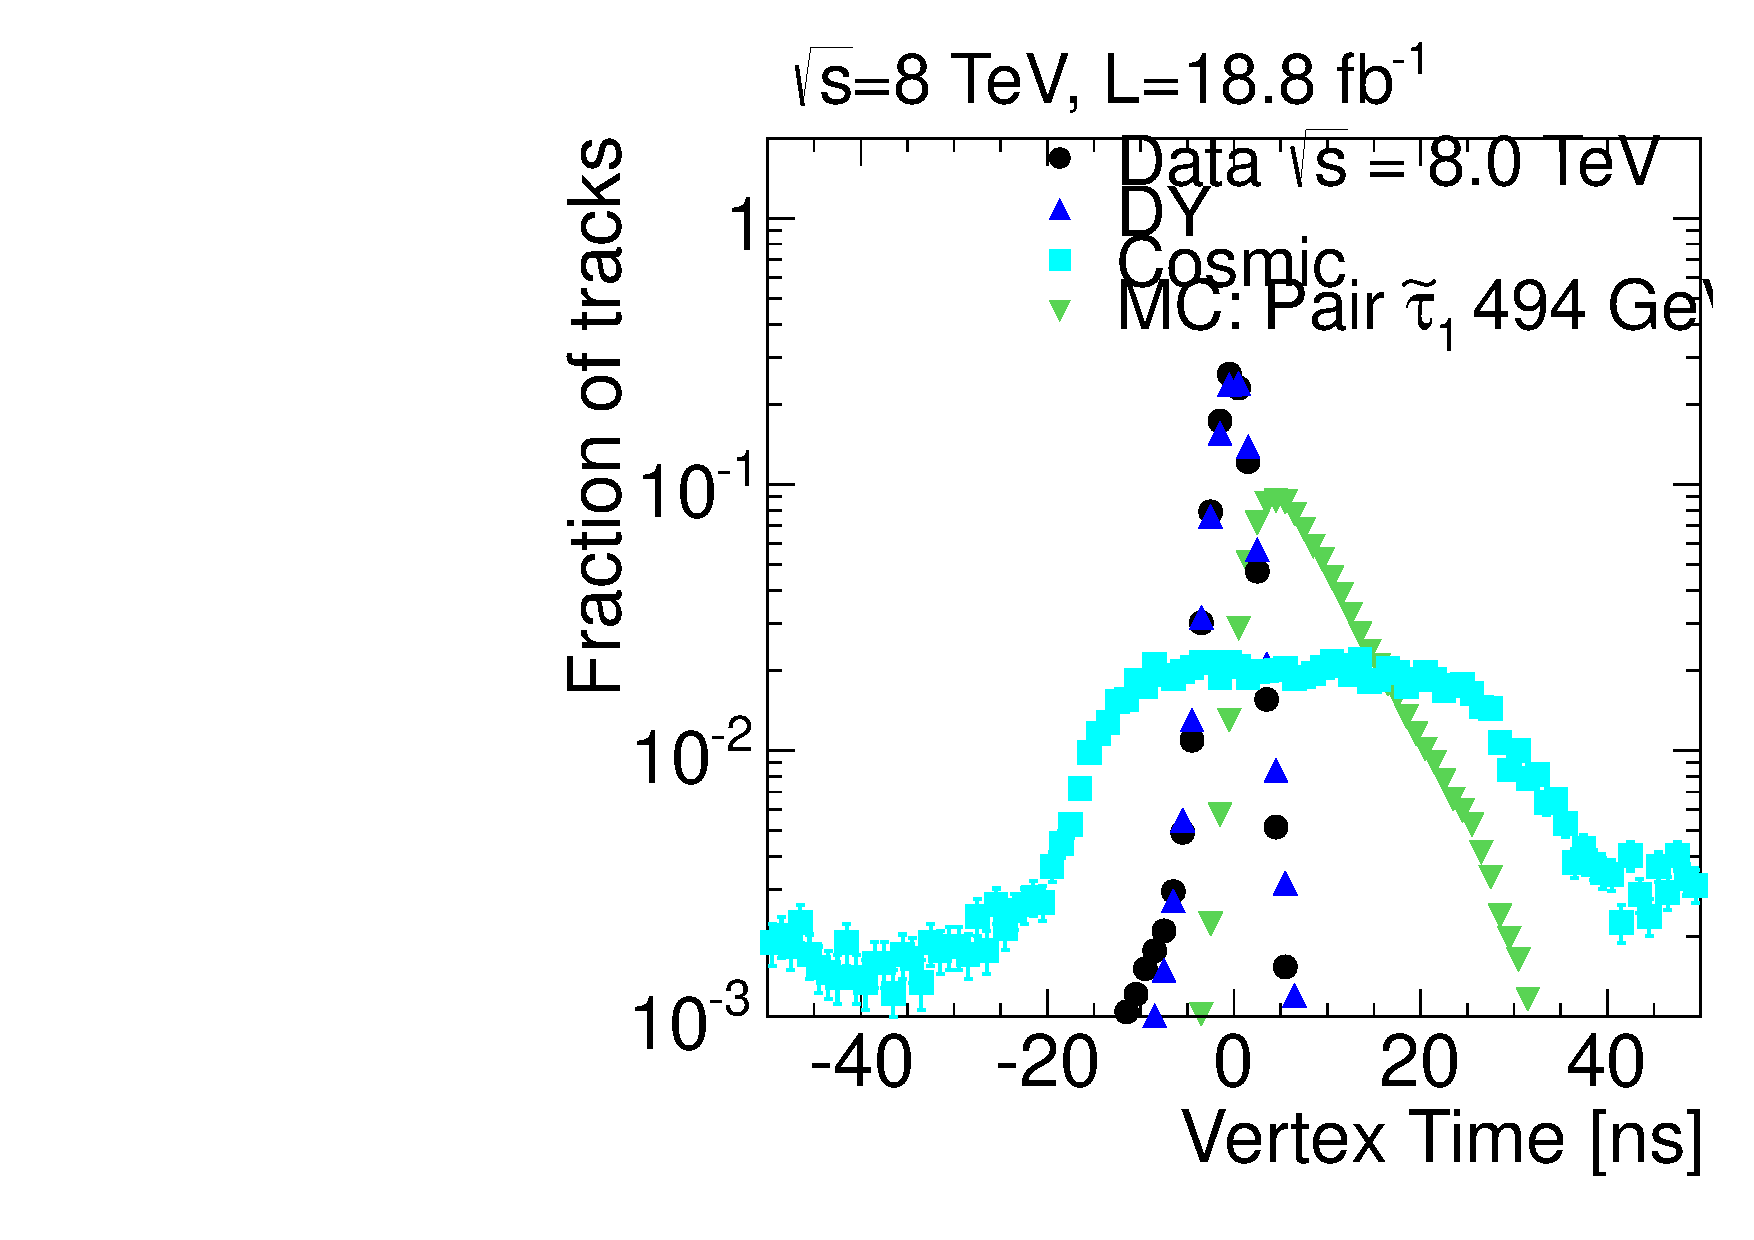
\includegraphics[width=0.44\textwidth]{figures/timing/Vertex}
      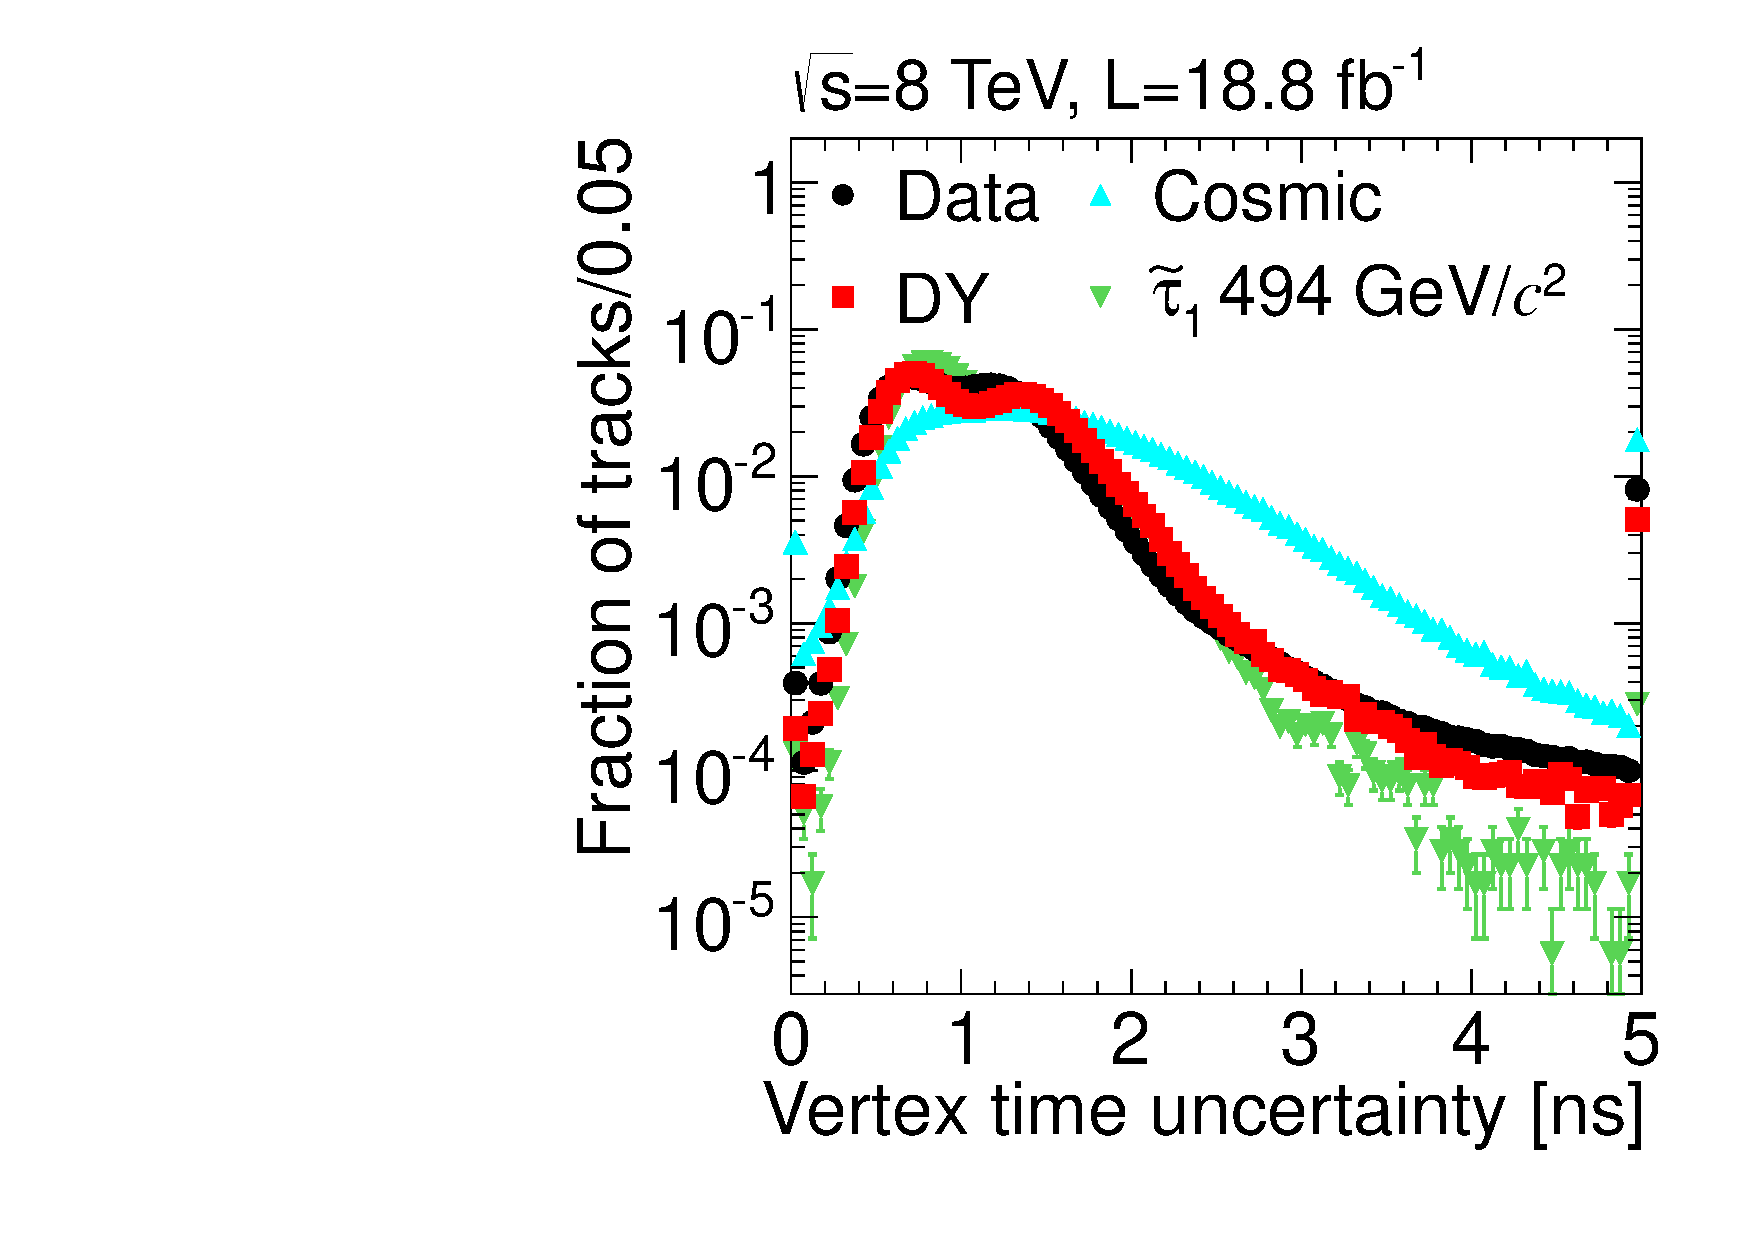
\includegraphics[width=0.44\textwidth]{figures/timing/VertexErr} \\
      \caption[Distribution of time at vertex and the uncertainty on time at vertex]
     {Distribution of time at vertex and the uncertainty on time at vertex for data,
simulated Drell-Yan production of photons and Z boson decaying to muons (DY), muons from cosmic rays, and simulated HSCPs
}
      \label{fig:vertextime}
  \end{center}
\end{figure}

The last variable, time at vertex out in, is similar but it assumes the particle is traveling into CMS, such that the parameter $t_0$ represents the time an incoming particle
would have crossed the interaction point. This can be an interesting property because tracks can be found in the inner tracker within a small time window so an incoming
cosmic reconstructed in the inner tracker would likely have a $t_0$ from this measurement near zero. 
The measurement assumes \invbeta\ = -1 reducing~\ref{eq:speed} to $t = -2 (d / c) + t_0$ which can be written to $t_0 = -2 (d / c) + t$ which makes it clear that
$t_0$ can be found as the average of this quantity with weights like the previous measurement. Figure~\ref{fig:vertexopptime} shows the distribution of this time
for the same three samples as above.

\begin{figure}
  \begin{center}
      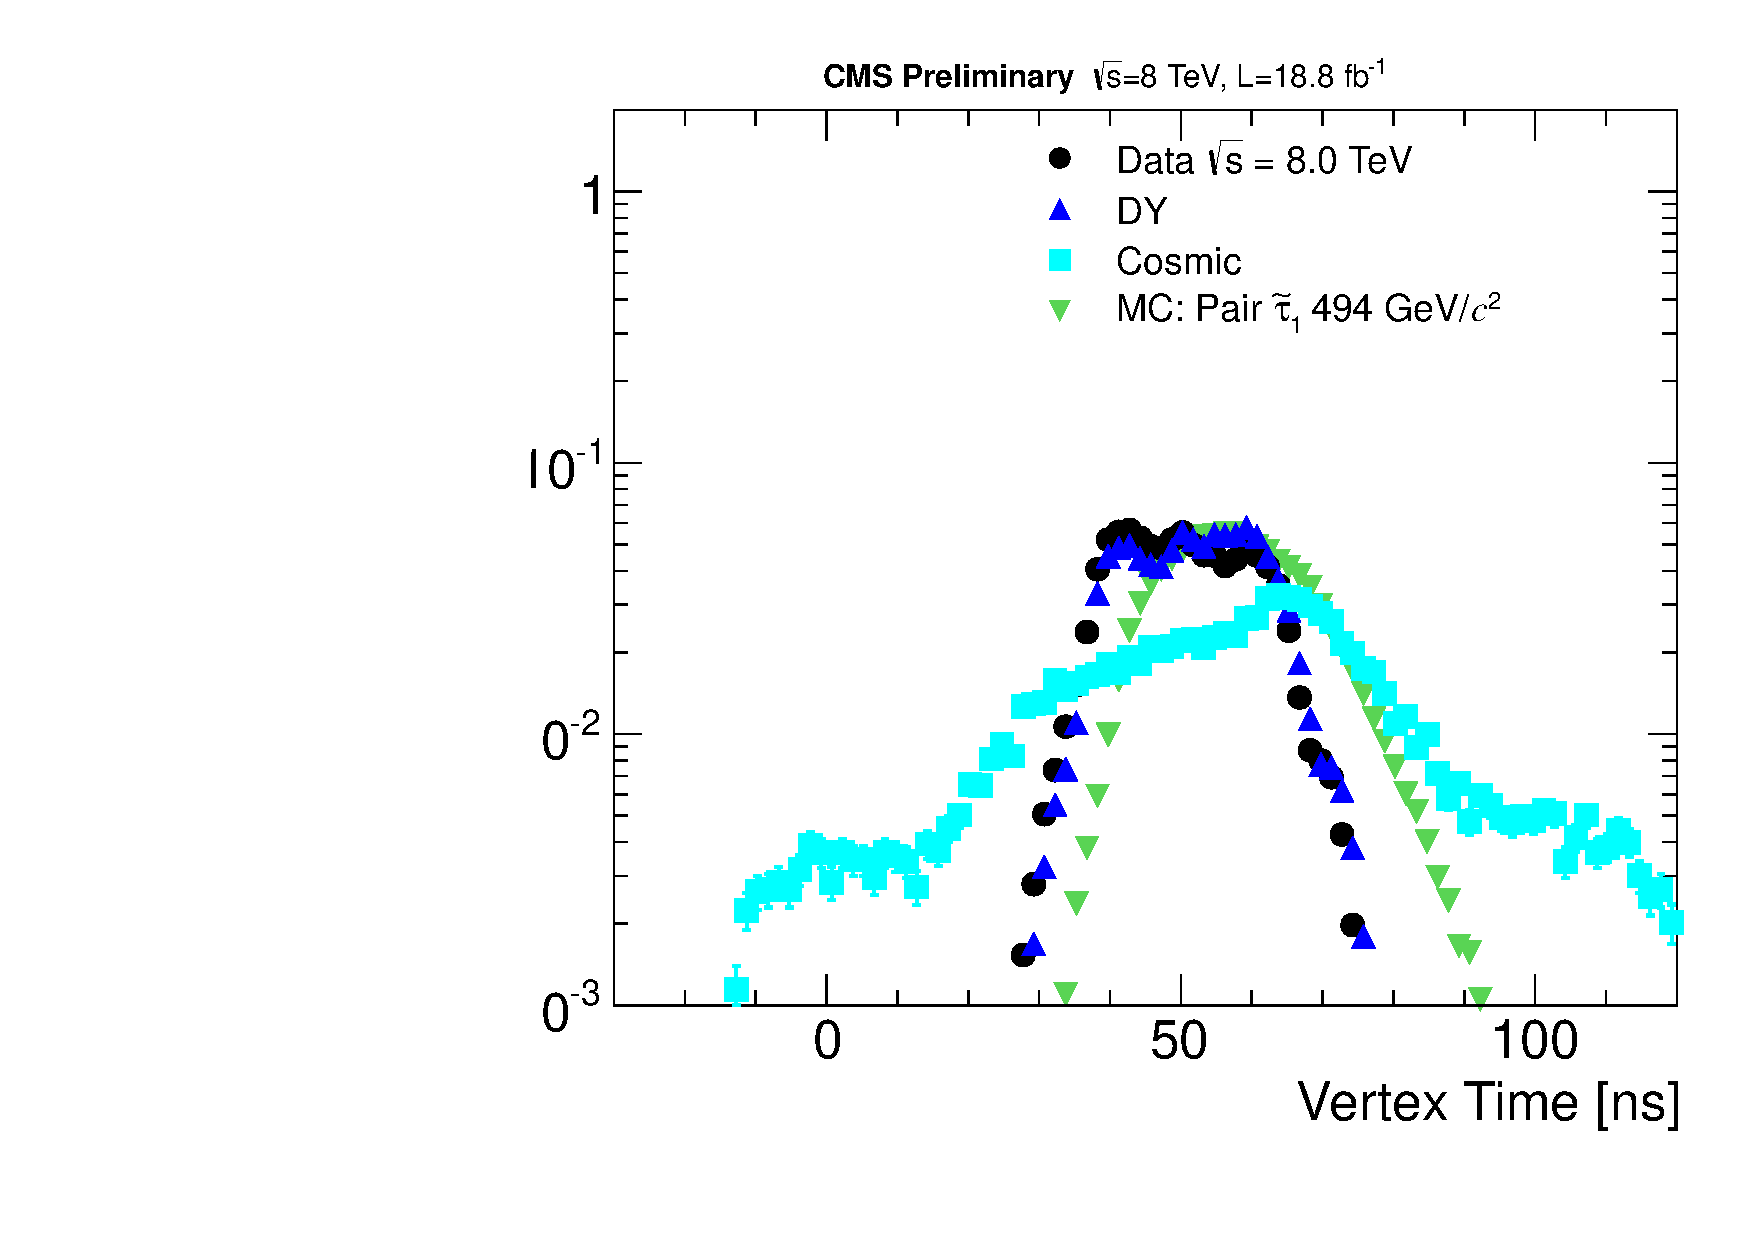
\includegraphics[width=0.44\textwidth]{figures/timing/VertexOpp}
      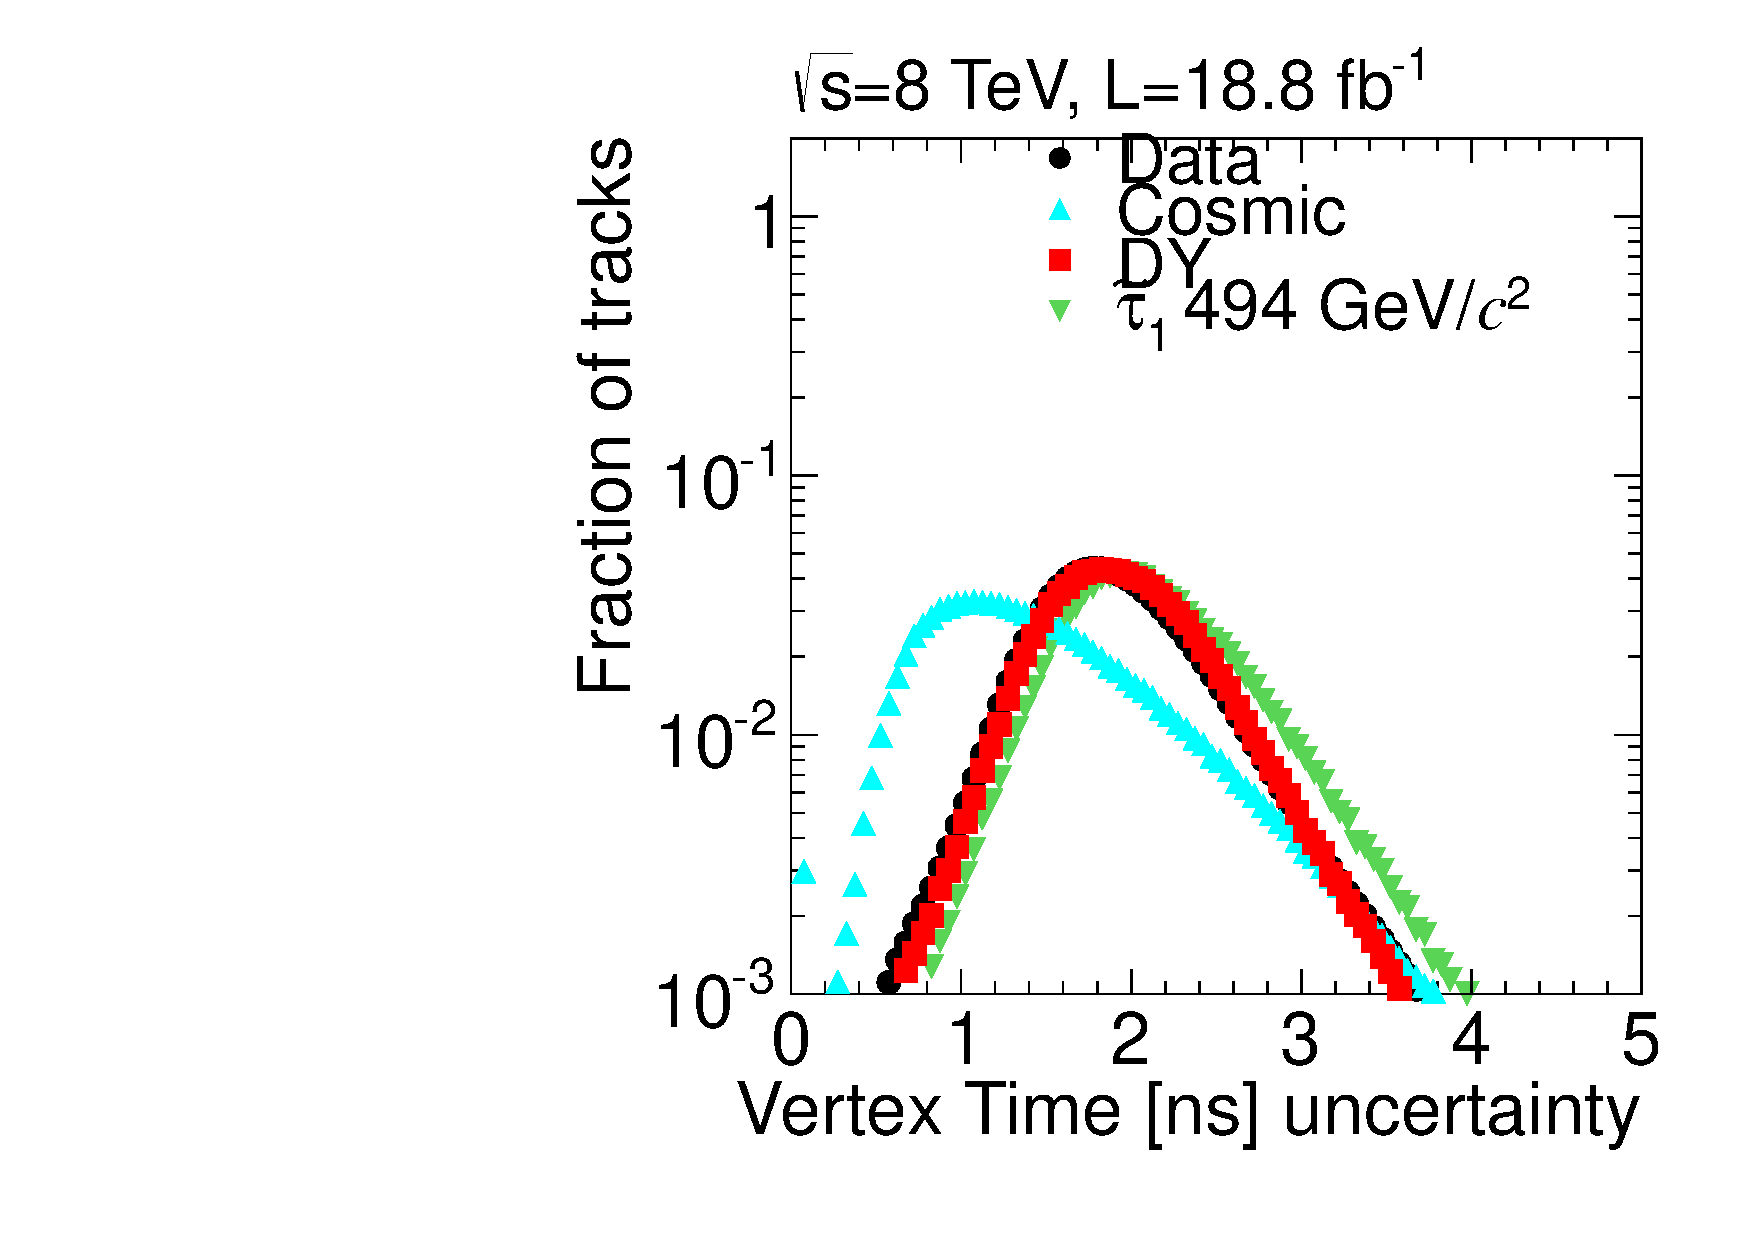
\includegraphics[width=0.44\textwidth]{figures/timing/VertexOppErr} \\
      \caption[Distribution of time at vertex out in and the uncertainty on time at vertex out in]
     {Distribution of time at vertex out in and the uncertainty on time at vertex out in for data,
simulated Drell-Yan production of photons and Z boson decaying to muons (DY), muons from cosmic rays, and simulated HSCPs
}
      \label{fig:vertexopptime}
  \end{center}
\end{figure}

The question may be asked why not to make a measurement without making any assumptions on $t_0$ or \invbeta. This was checked but it was found to have
resolution worse by more than an order of magnitude and very little discrimanatory power.
This is because the assumptions in the previous measurements allowed all of them to use information
related to the beam spot, which is approximately three times as far away from the innermost part of the muon system as the outermost part is to the innermost part.
The last two measurements both assumed an error free propagation of the time in the muon system to the interaction point while the \invbeta\ measurement
added a new point at the interaction point with t = 0. This assumption free measurement is not used for any purpose in CMS.

%\section{Timing in simulation} Maybe

%\section{Conclusion}
